\chapter{Comparison and Evaluation}
\label{sec:comparison_and_evaluation}

In this section, we compare the two developed fuzzy tuning approaches with other tuning techniques present in AutoPas and evaluate their performance.

\medskip

\noindent To measure the performance of the fuzzy tuning strategy, we use the scenarios present in \texttt{md\_flexible} and compare the results with the other tuning strategies present in AutoPas. The benchmarks are run on the CoolMUC-2\footnote{\label{CoolMucSpecs}CoolMUC-2 is a supercomputer located at the Leibniz Supercomputing Centre in Garching, Germany. It consists of 812 Haswell-based nodes with 14 cores each. As a result of hyperthreading, each node supports up to 28 threads. More information can be found at \url{https://doku.lrz.de/coolmuc-2-11484376.html}} cluster and are repeated with 1, 12, 24, and 28 threads. We use the \texttt{timeSpentCalculatingForces} metric to evaluate the performance of the tuning strategies as it gives a good indication of the overall performance of the simulation.


\section{Exploding Liquid Benchmark (Included in Training Data)}
\label{sec:explodingLiquidBenchmark}

The exploding liquid benchmark simulates a high-density liquid that expands outwards as the simulation progresses. As the data of this scenario was included in the training data, we expect the fuzzy tuning technique to perform well.

The plot in \autoref{fig:explodingTimings_1thread} shows the time spent calculating the forces for each tuning strategy throughout the simulation. We only include the benchmark results using one thread for brevity, as all thread counts resulted in very similar behavior.

The plot shows that both fuzzy tuning strategies perform close to optimal and show very stable force calculation times throughout the simulation. All other tuning strategies show a much higher variance caused by significantly more testing and worse configurations during the tuning phases.

To show the differences between the strategies in more detail, we also include a boxplot of the time spent calculating the forces for each tuning strategy based on the current phase in \autoref{fig:explodingLiquidBoxplot_1thread}. All tuning strategies show similar timings during the simulation phases, as they eventually found a close-to-optimal configuration during the tuning phase. The tuning phases, however, differ drastically: All rule-based strategies (Fuzzy tuning and Rule-Based Tuning) tend to perform better in tuning phases and evaluate fewer bad configurations, as the rule files should discourage the evaluation of such configurations.

The last plot in \autoref{fig:explodingLiquidTotalTime_1thread} shows the total time spent calculating the forces for each tuning strategy, again divided into simulation and tuning time. The fuzzy tuning strategies have the lowest total time, with practically no time spent in the tuning phases. In contrast, all other strategies spend about 50\% of their total time in the tuning phases.

Both fuzzy tuning approaches perform similarly and are by far the best-performing strategies, achieving a speedup of $\frac{t_{\text{FullSearch}}}{t_{\text{Fuzzy[Components]}}} = \frac{32.5s}{16.6s} \approx 1.96$ and $\frac{t_{\text{FullSearch}}}{t_{\text{Fuzzy[Suitability]}}} = \frac{32.5s}{20.3s} \approx 1.60$, respectively.

The low tuning overhead is the most significant contributor to the performance of the fuzzy tuning strategies. The tuning phases of the fuzzy tuning strategies are very short and mainly consist of evaluating already known suitable configurations, which causes very little overhead during the tuning phases. This is in contrast to the classical tuning strategies, which evaluate many bad configurations during the tuning phases, causing a significant slowdown. Those bad configurations are the main reason for the poor performance of the classical tuning strategies.

We observe that the suitability approach performs slightly worse during simulation phases compared to all other strategies. This is caused by the suitability approach not finding the optimal configuration during the first tuning phases. In later tuning phases, however, the suitability approach always succeeds in finding the optimal configuration. Even with this slight error in the suitability approach, it still performed better than all classical strategies.


\section{Spinodal Decomposition MPI (Related to Training Data)}

The spinodal decomposition benchmark simulates an unstable liquid that separates into two phases, each having different characteristics. To improve the performance of the simulation, we used four different MPI ranks, each running on 14 threads to simulate the scenario.

As a full Spinodal Decomposition run with just one rank was included in the training data, and the scenario is very homogeneous, we expect the fuzzy tuning strategies to also perform well in the smaller regions handled by the individual MPI ranks, especially as the rule files only contain \emph{relative} rules, that should be unaffected by rescaling the scenario.

The plot in \autoref{fig:spinodalTimings_14thread} shows the time spent calculating the forces for each tuning strategy throughout the simulation. For brevity, we again only include the benchmark results for the 0th MPI rank, as the results for the other MPI ranks are nearly identical. This time, we see a difference in both fuzzy tuning strategies, as the component tuning approach performs way better than the suitability approach for most of the simulation.

From \autoref{fig:spinodalTimings_14thread}, we see that the suitability approach performed the worst during most simulation phases, as it never found the true optimal configuration during the tuning phases. This is primarily caused by the suitability threshold of 10\% being too low for this scenario. The low threshold caused the suitability approach to be overly optimistic in its predictions and resulted in very few configurations actually being evaluated during the tuning phases. The predicted configurations were not bad, as shown in \autoref{fig:spinodalBoxplot_14thread}, but didn't include the optimal configuration. \autoref{sec:suitabilityThreshold} will investigate the suitability threshold's effect on the simulation's performance in more detail.

\autoref{fig:spinodal_14thread} shows that the component tuning approach again performs best, with a speedup of $\frac{t_{\text{FullSearch}}}{t_{\text{Fuzzy[Components]}}} = \frac{2236.1s}{1650.3s} \approx 1.35$. Surprisingly, the suitability approach performed reasonably well despite never finding the optimal configuration, mainly due to basically no time wasted during the tuning phases. In particular it achieves a speedup of $\frac{t_{\text{FullSearch}}}{t_{\text{Fuzzy[Suitability]}}} = \frac{2236.1s}{1846.1s} \approx 1.21$ which places it on the third place. This shows the importance of efficient tuning phases, as they can cause tremendous overhead if not done correctly.

\newpage

\begin{figure}[H]
    \centering

    \begin{subfigure}[c]{\textwidth}
        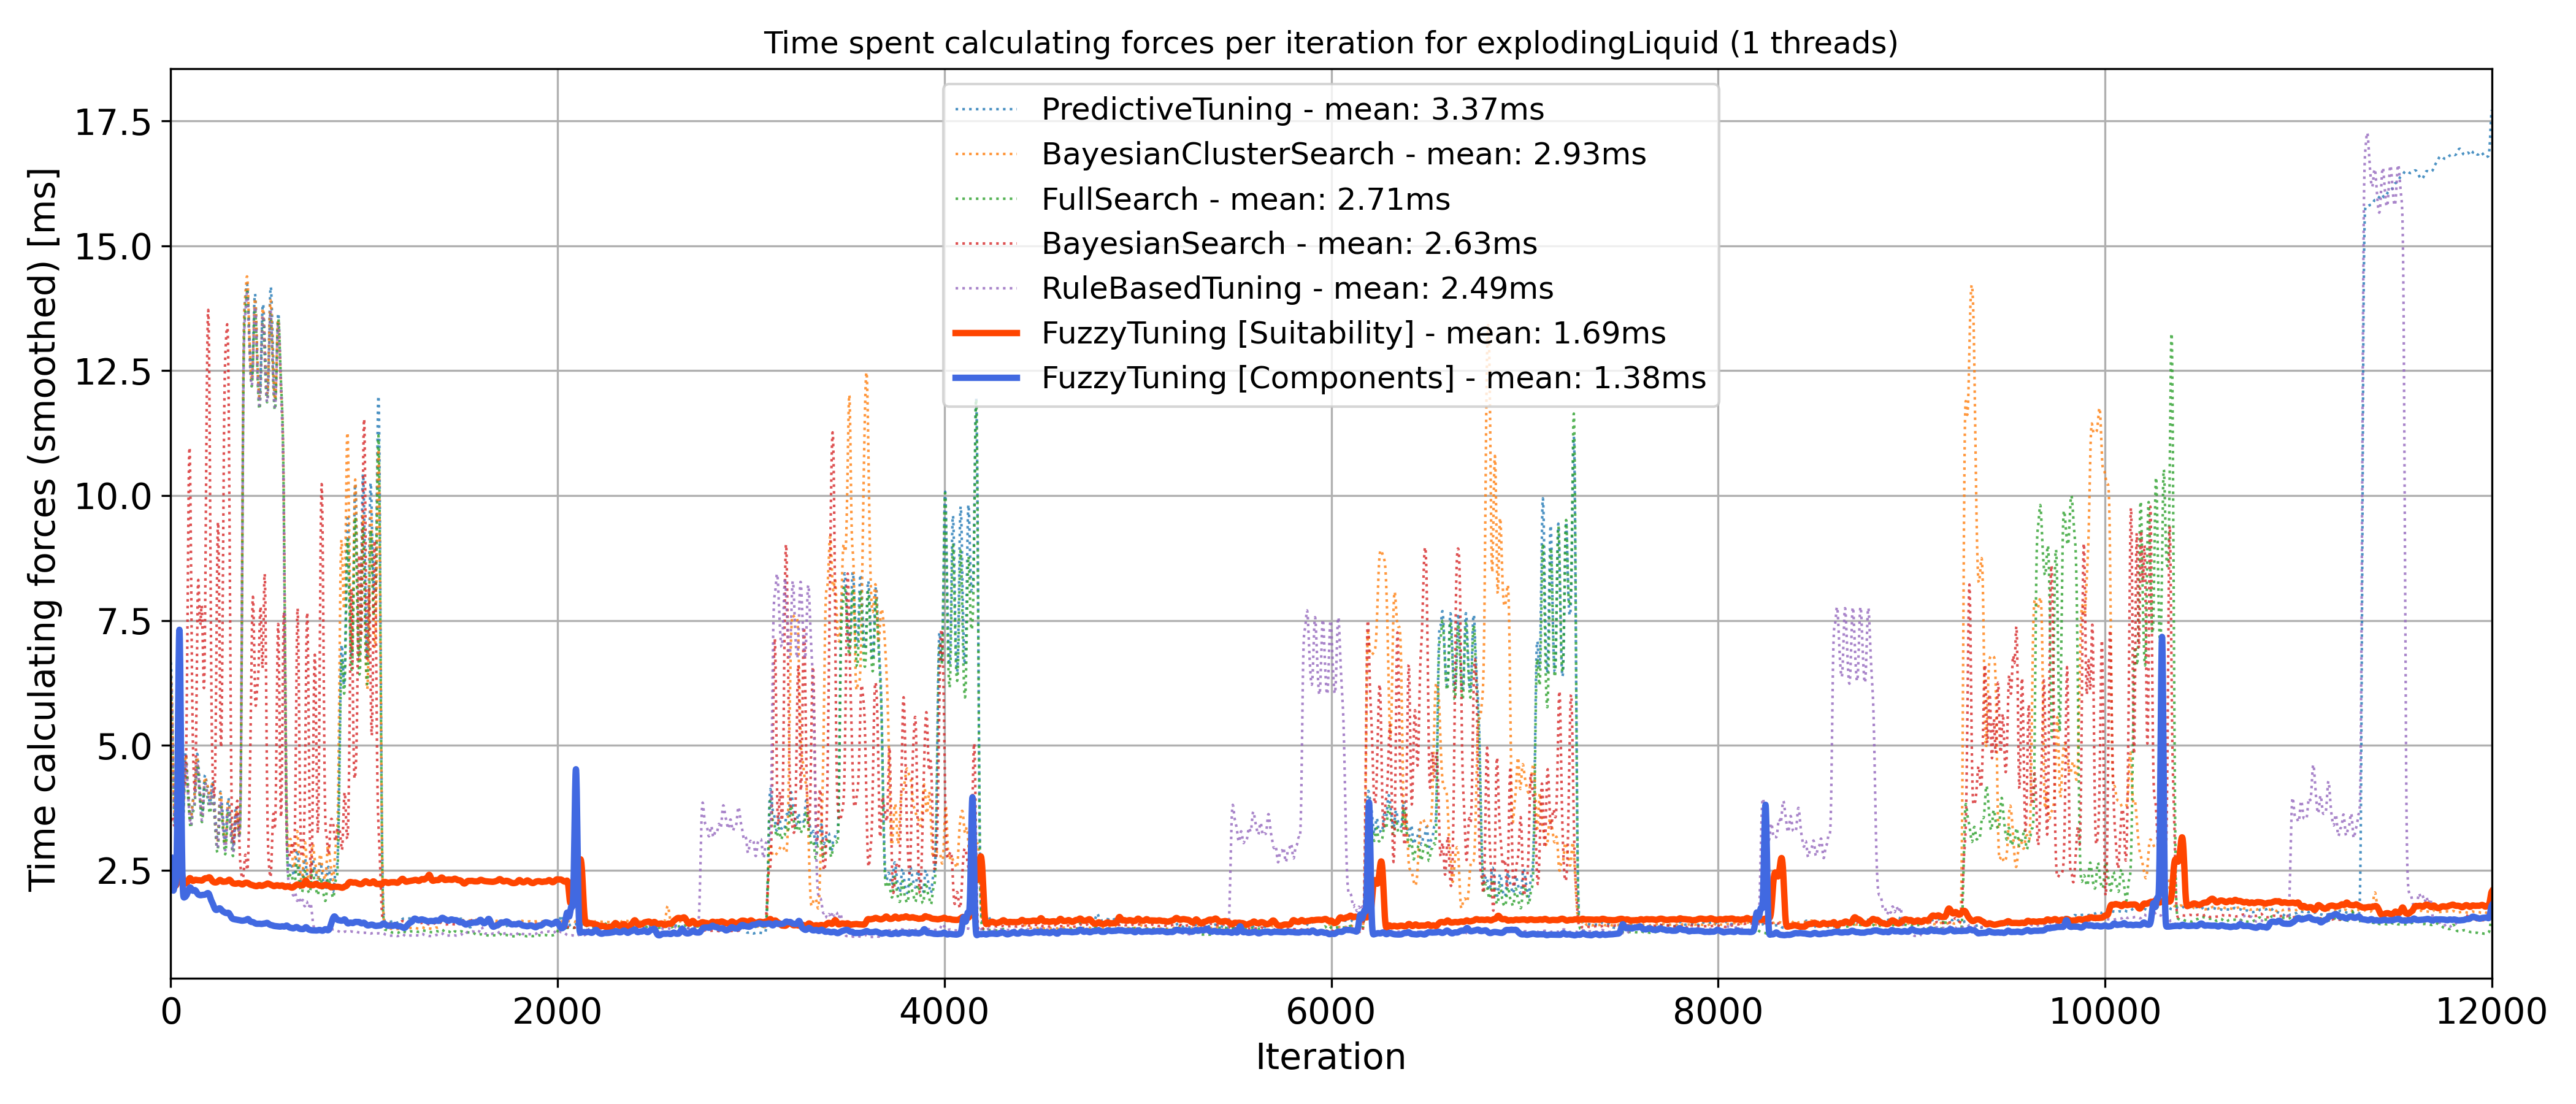
\includegraphics[width=\columnwidth,trim={0cm 0cm 0cm 0.9cm},clip]{figures/Benchmark/ExplodingLiquid/timing_explodingLiquid_1.png}
        \caption{}
        \label{fig:explodingTimings_1thread}
    \end{subfigure}


    \begin{subfigure}[c]{\textwidth}
        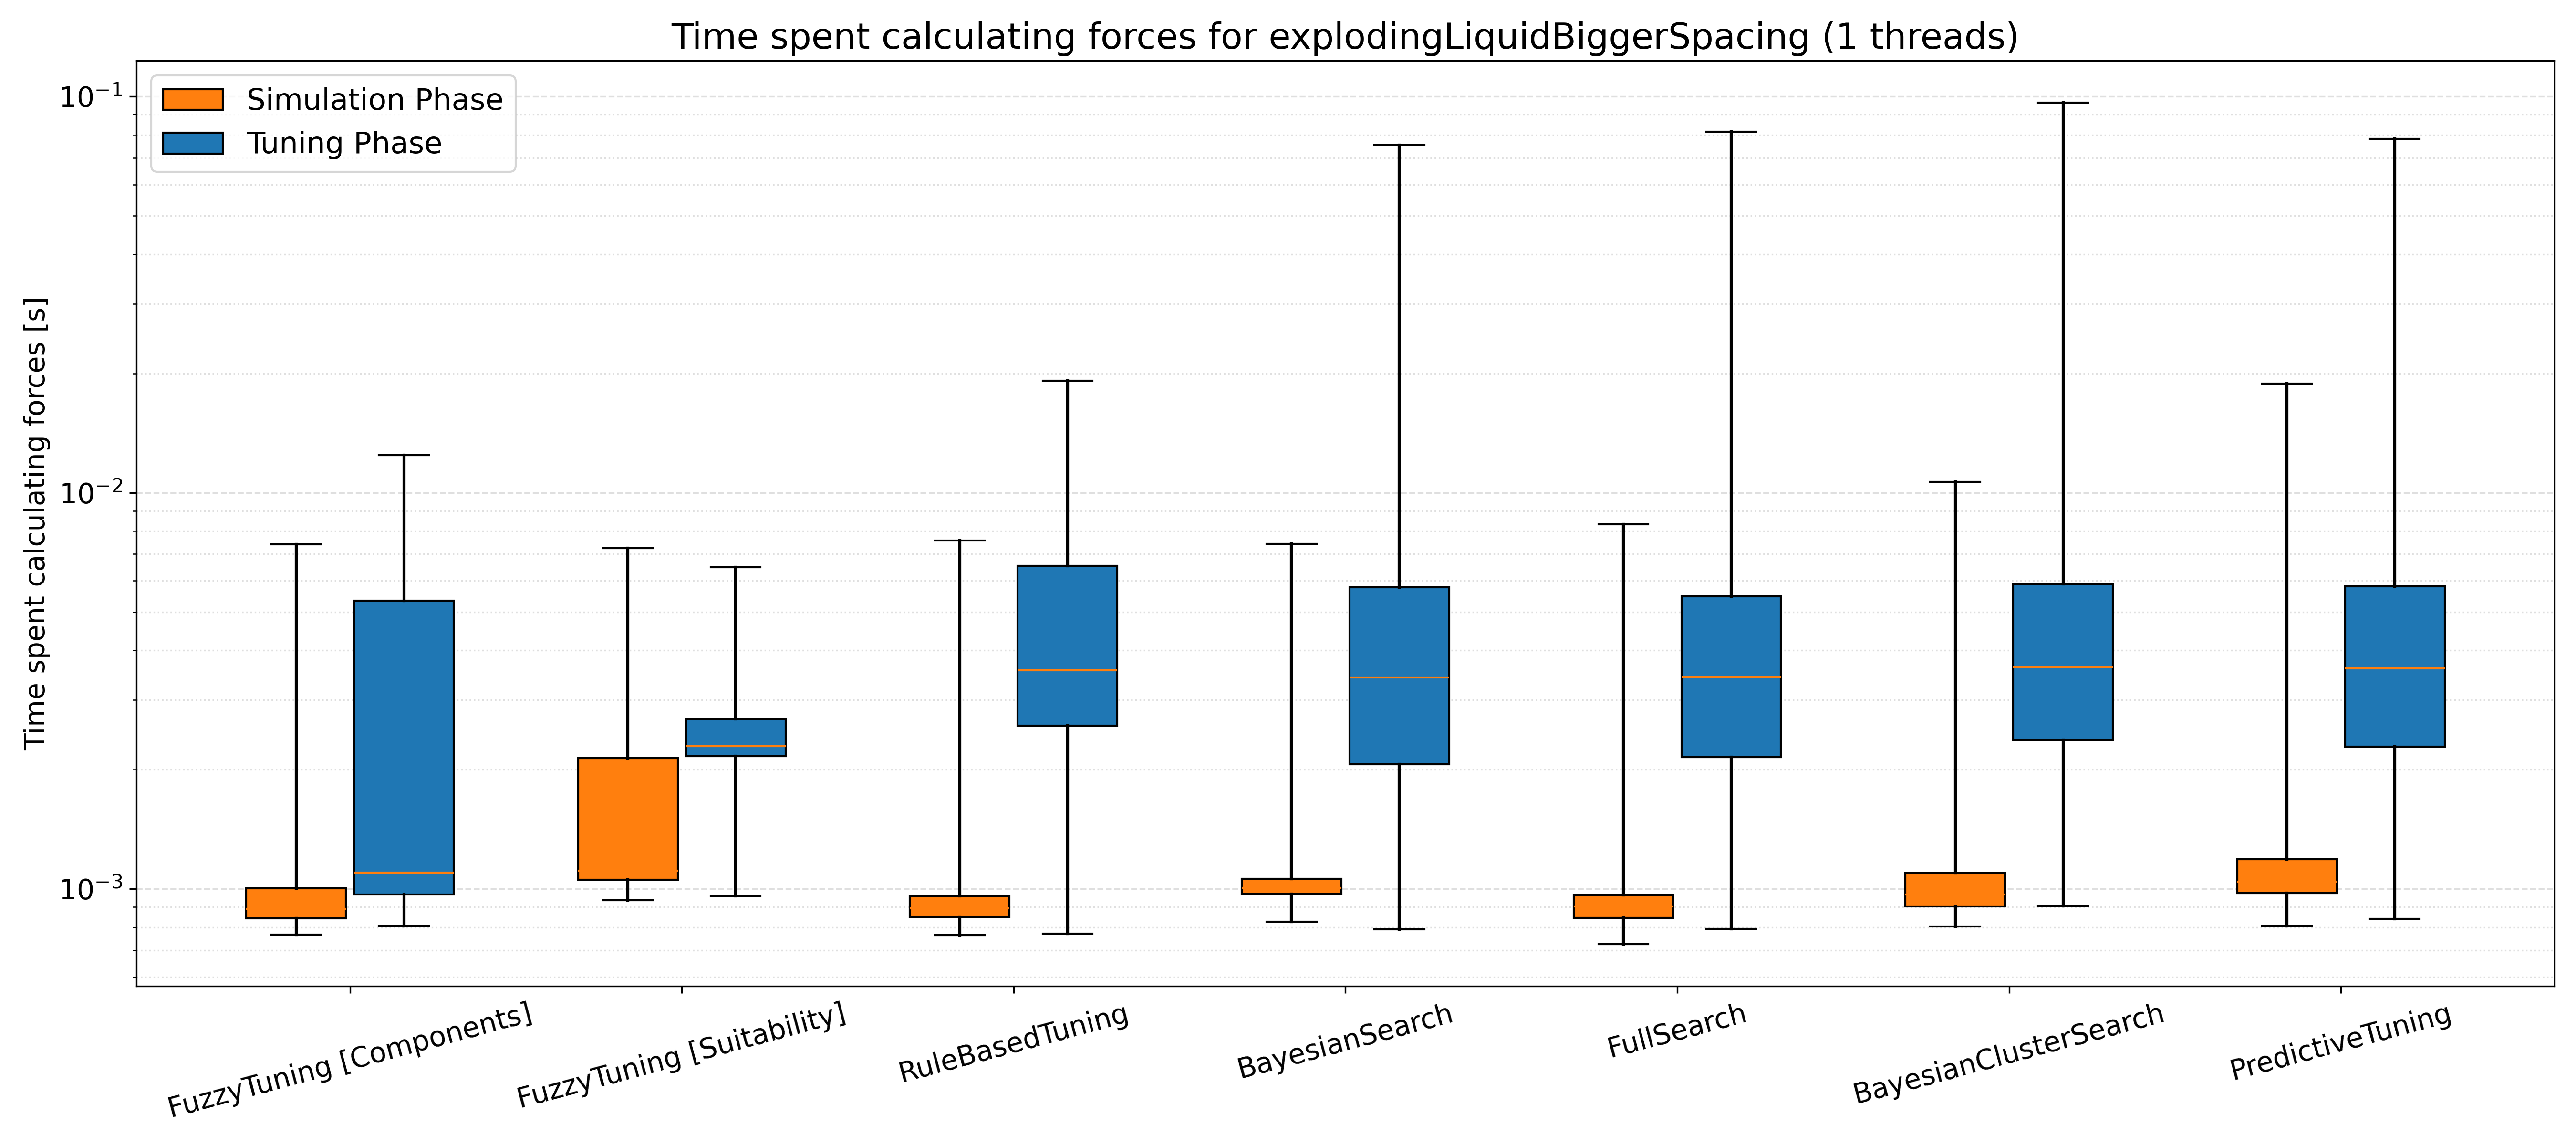
\includegraphics[width=\columnwidth,trim={0cm 0.5cm 0cm 1cm},clip]{figures/Benchmark/ExplodingLiquid/boxplot_explodingLiquid_1.png}
        \caption{}
        \label{fig:explodingLiquidBoxplot_1thread}
    \end{subfigure}

    \begin{subfigure}[b]{\textwidth}
        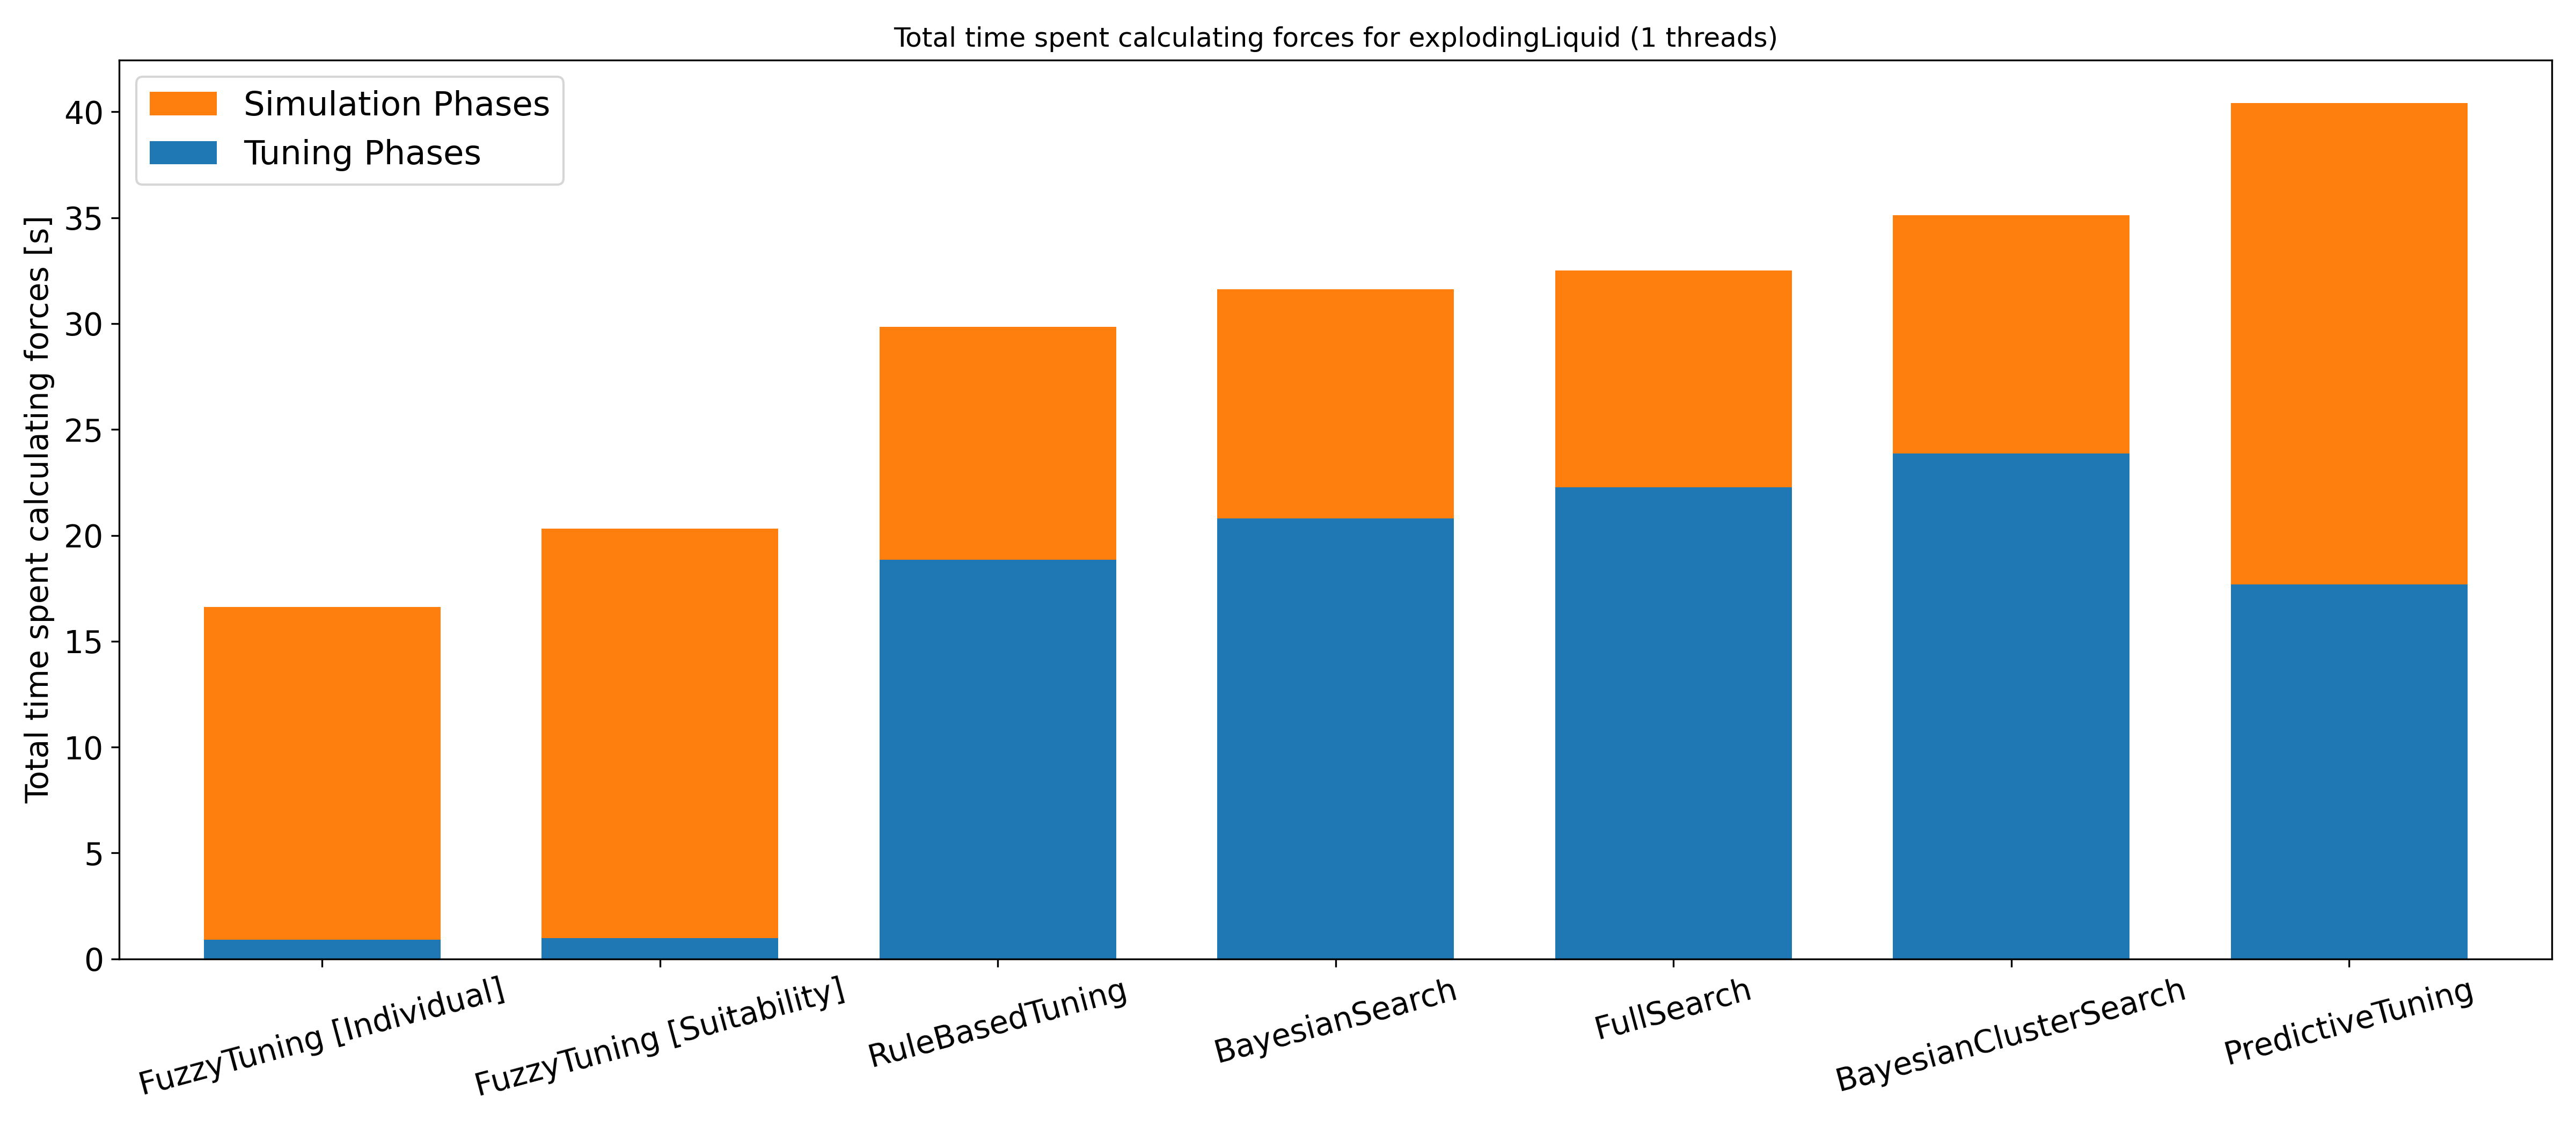
\includegraphics[width=\columnwidth,trim={0cm 0.5cm 0cm 0.9cm},clip]{figures/Benchmark/ExplodingLiquid/total_time_explodingLiquid_1.png}
        \caption{}
        \label{fig:explodingLiquidTotalTime_1thread}
    \end{subfigure}


    \caption[Benchmark Results for the Exploding Liquid Scenario]{Exploding Liquid benchmark with 1 thread. (a) Time spent calculating forces for every iteration. (b) Boxplots of time spent calculating forces divided into tuning- and simulation phases. (c) Total time spent calculating forces for tuning- and simulation phases. The Suitability approach uses a non-optimal threshold of 10\% (see \autoref{sec:suitabilityThreshold}).}
    \label{fig:explodingLiquid_1thread}
\end{figure}

\begin{figure}[H]
    \centering

    \begin{subfigure}[c]{\textwidth}
        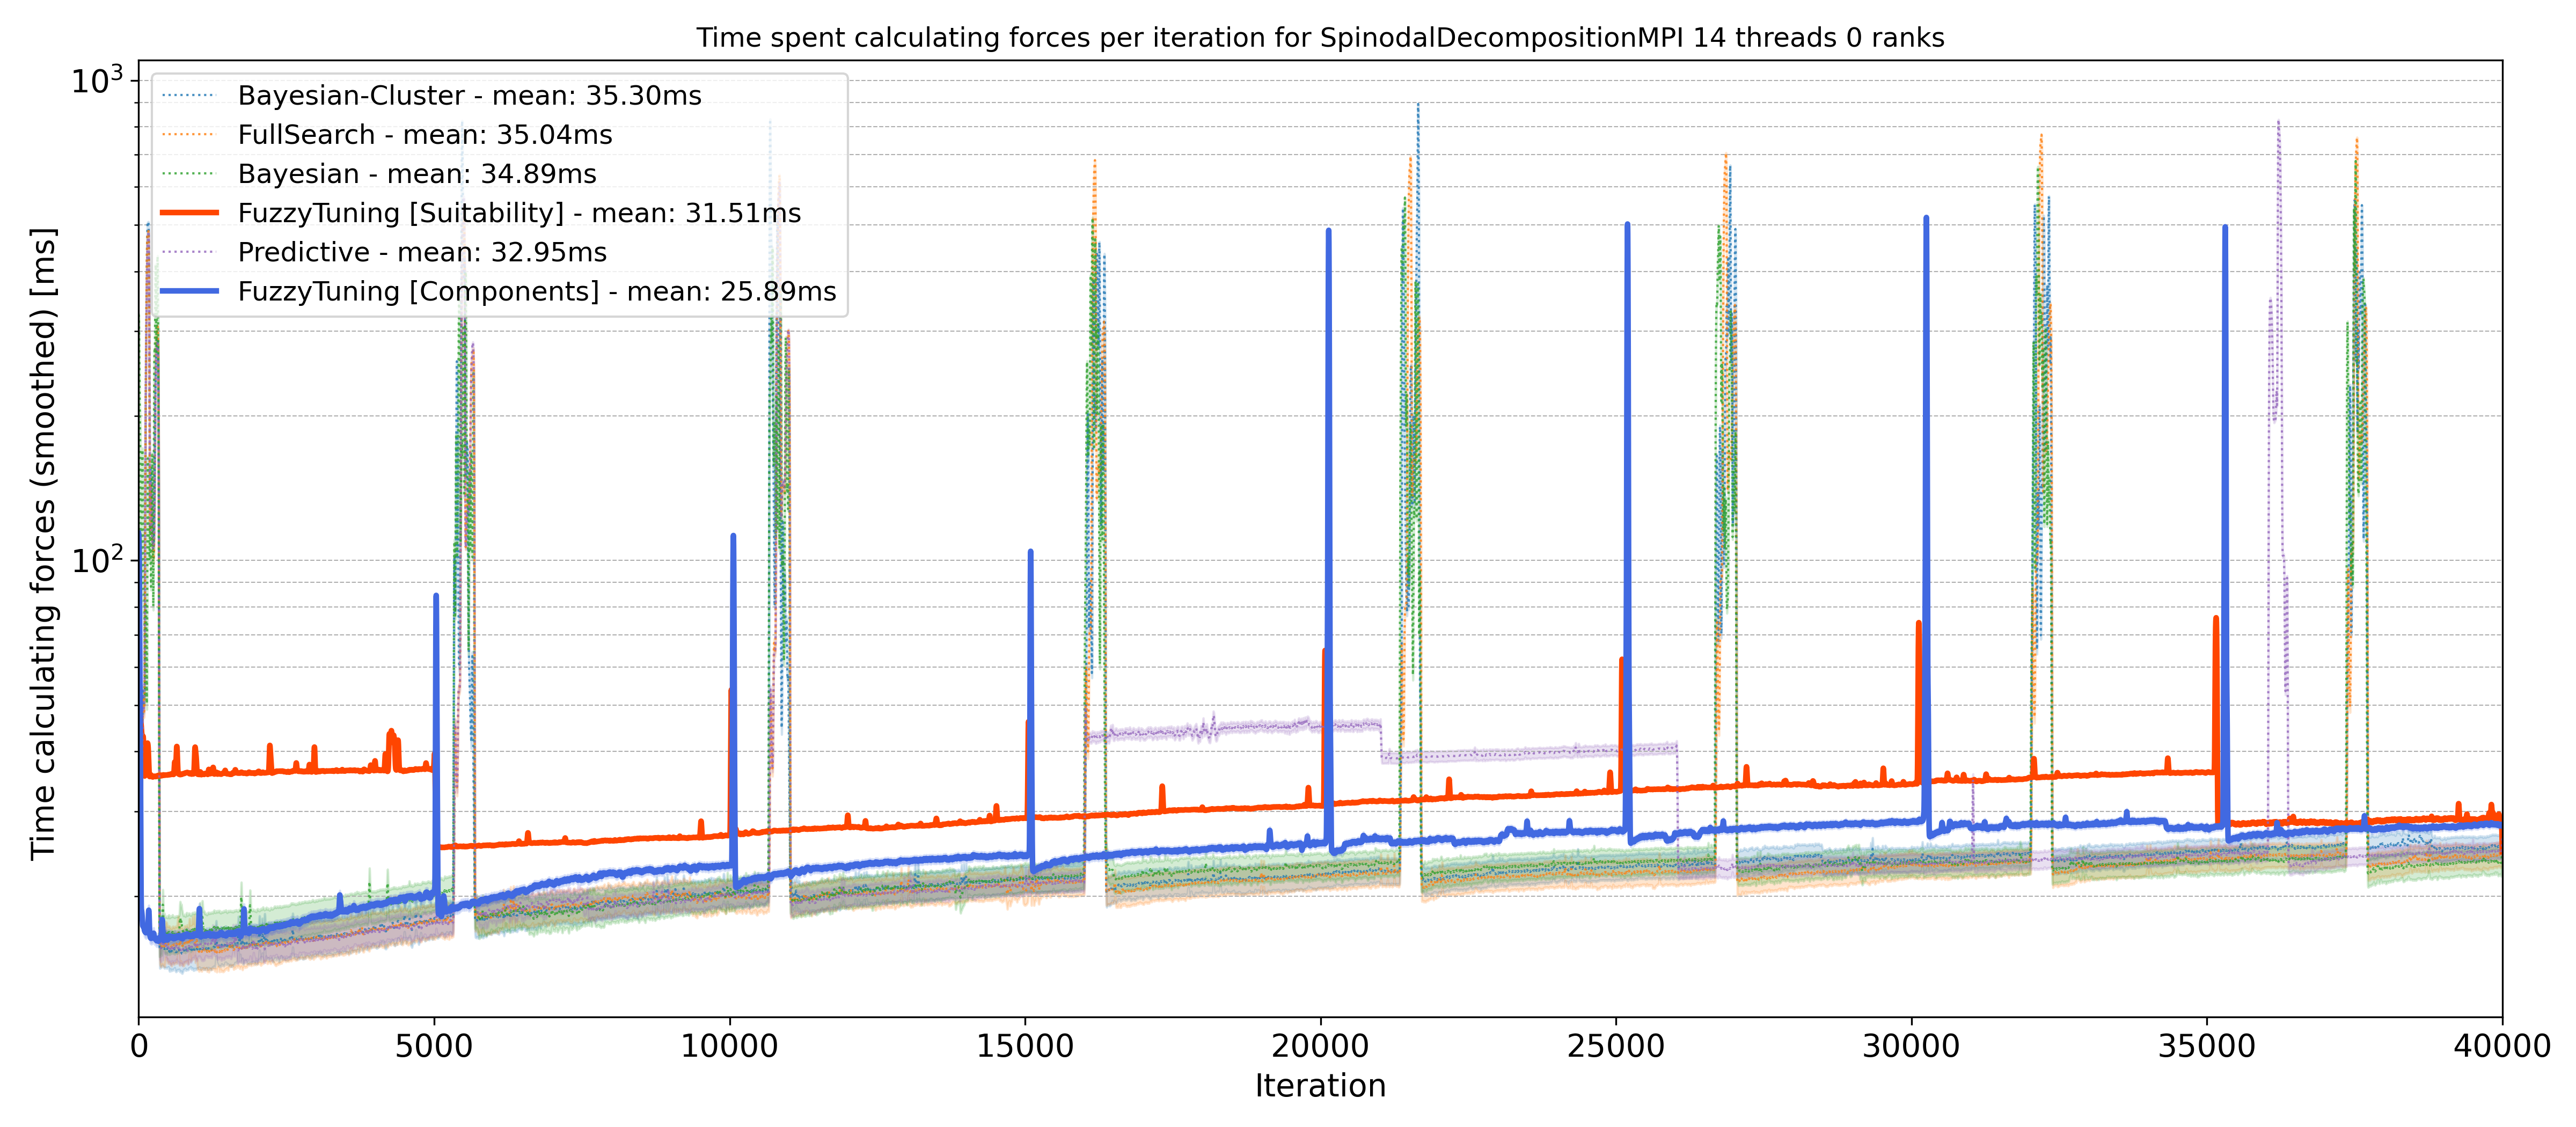
\includegraphics[width=\columnwidth,trim={0cm 0.4cm 0cm 0.9cm},clip]{figures/Benchmark/SpinodalDecompositionMPI/SpinodalDecompositionMPI_timings_SpinodalDecompositionMPI_14_0.png}
        \caption{}
        \label{fig:spinodalTimings_14thread}
    \end{subfigure}


    \begin{subfigure}[c]{\textwidth}
        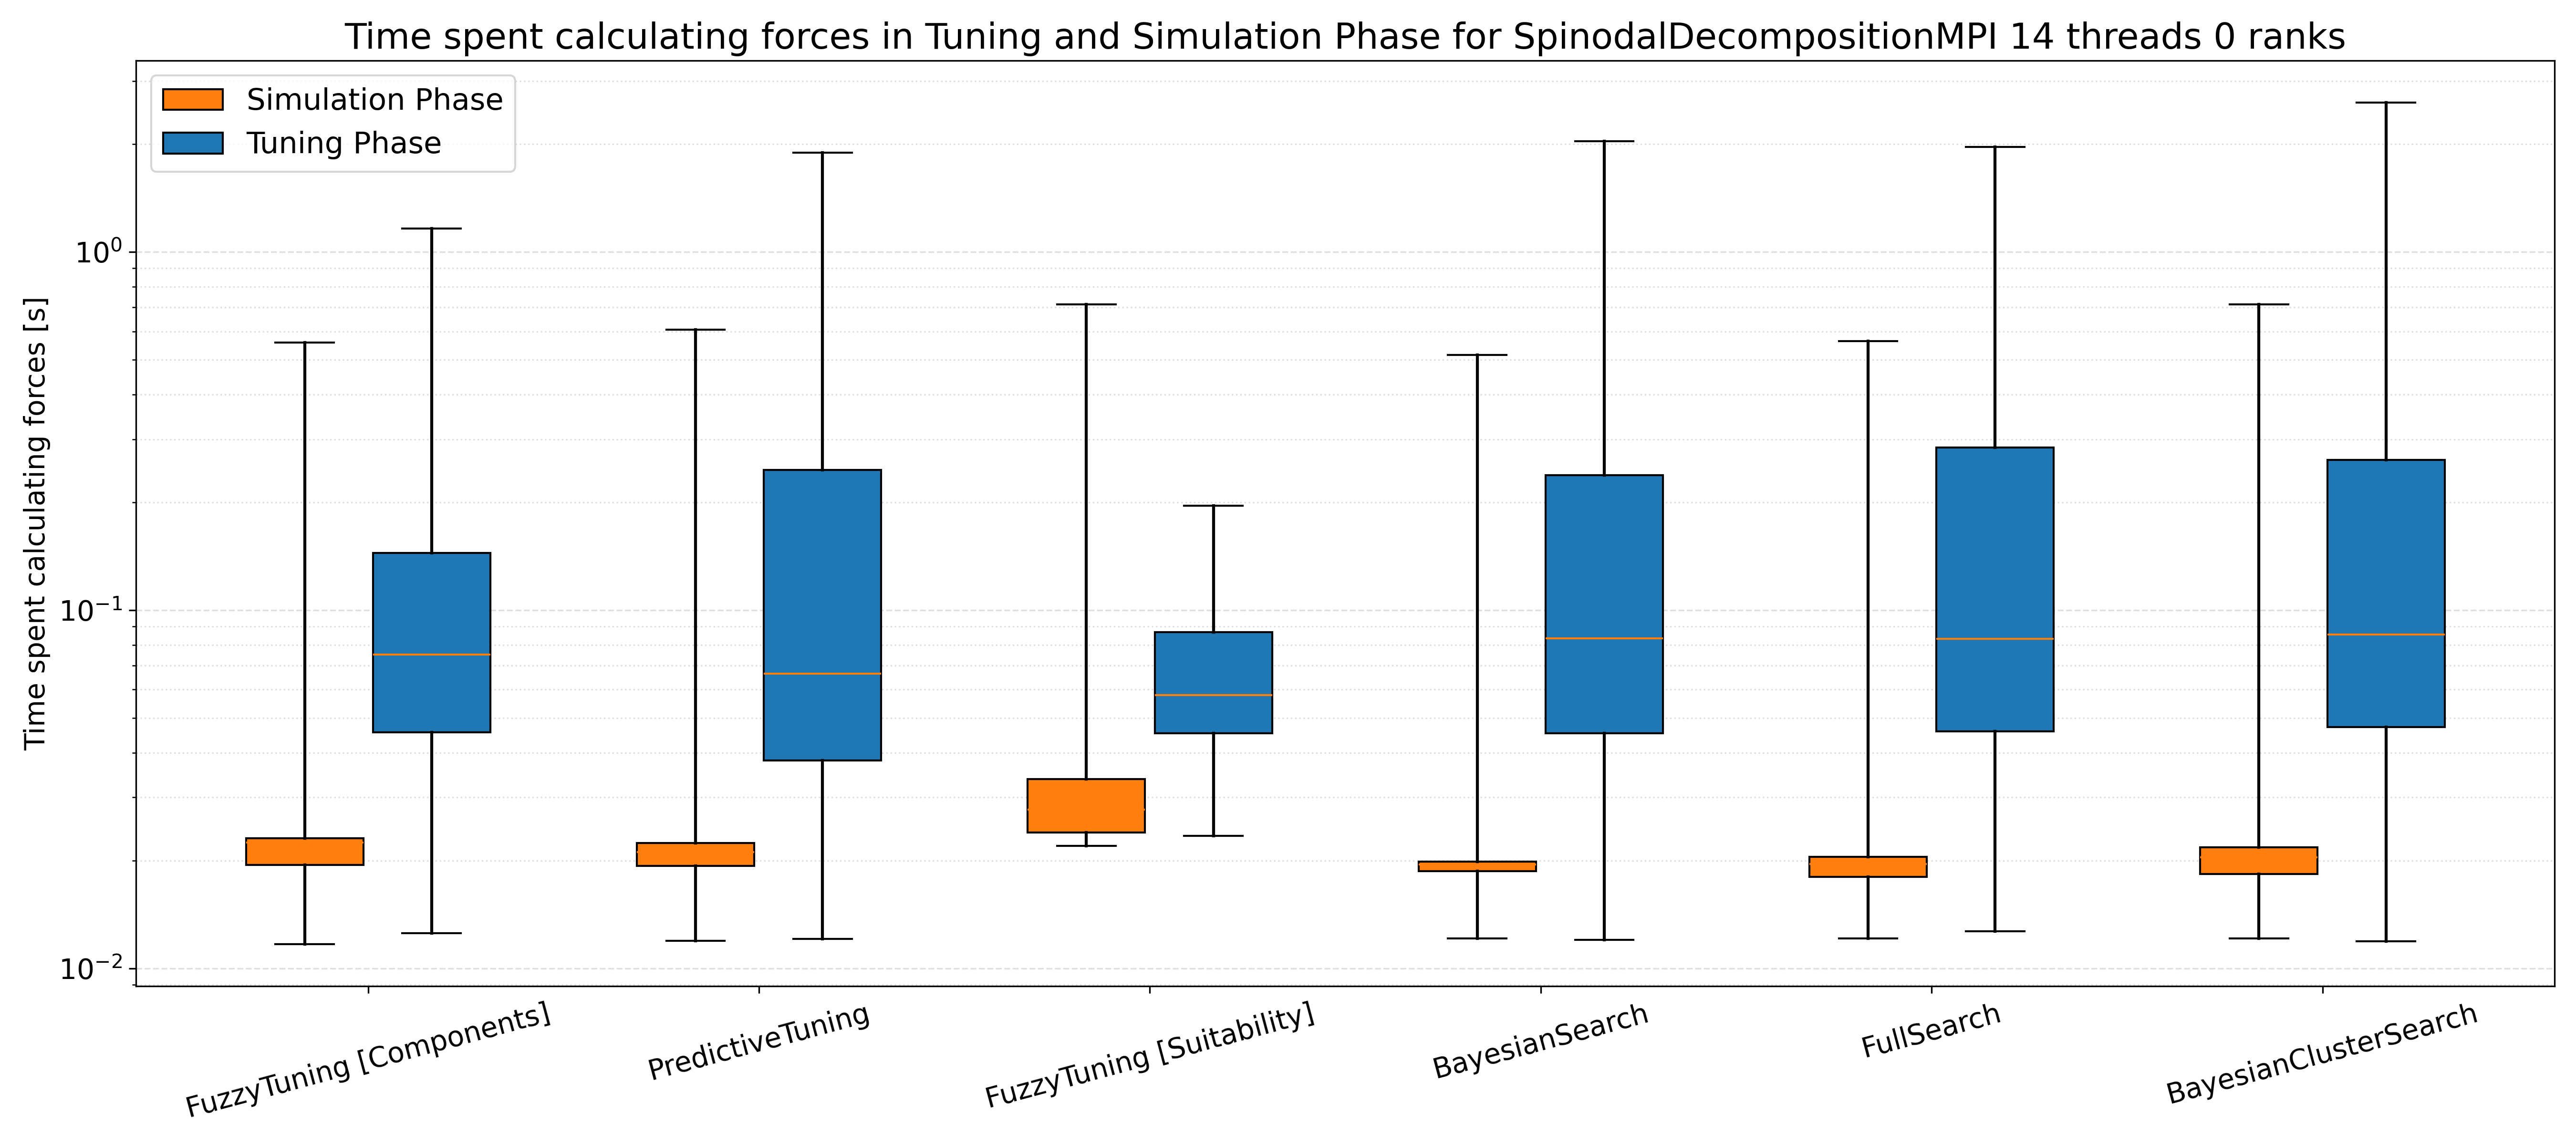
\includegraphics[width=\columnwidth,trim={0cm 0.5cm 0cm 1cm},clip]{figures/Benchmark/SpinodalDecompositionMPI/SpinodalDecompositionMPI_timings_boxplot_SpinodalDecompositionMPI_14_0.png}
        \caption{}
        \label{fig:spinodalBoxplot_14thread}
    \end{subfigure}

    \begin{subfigure}[b]{\textwidth}
        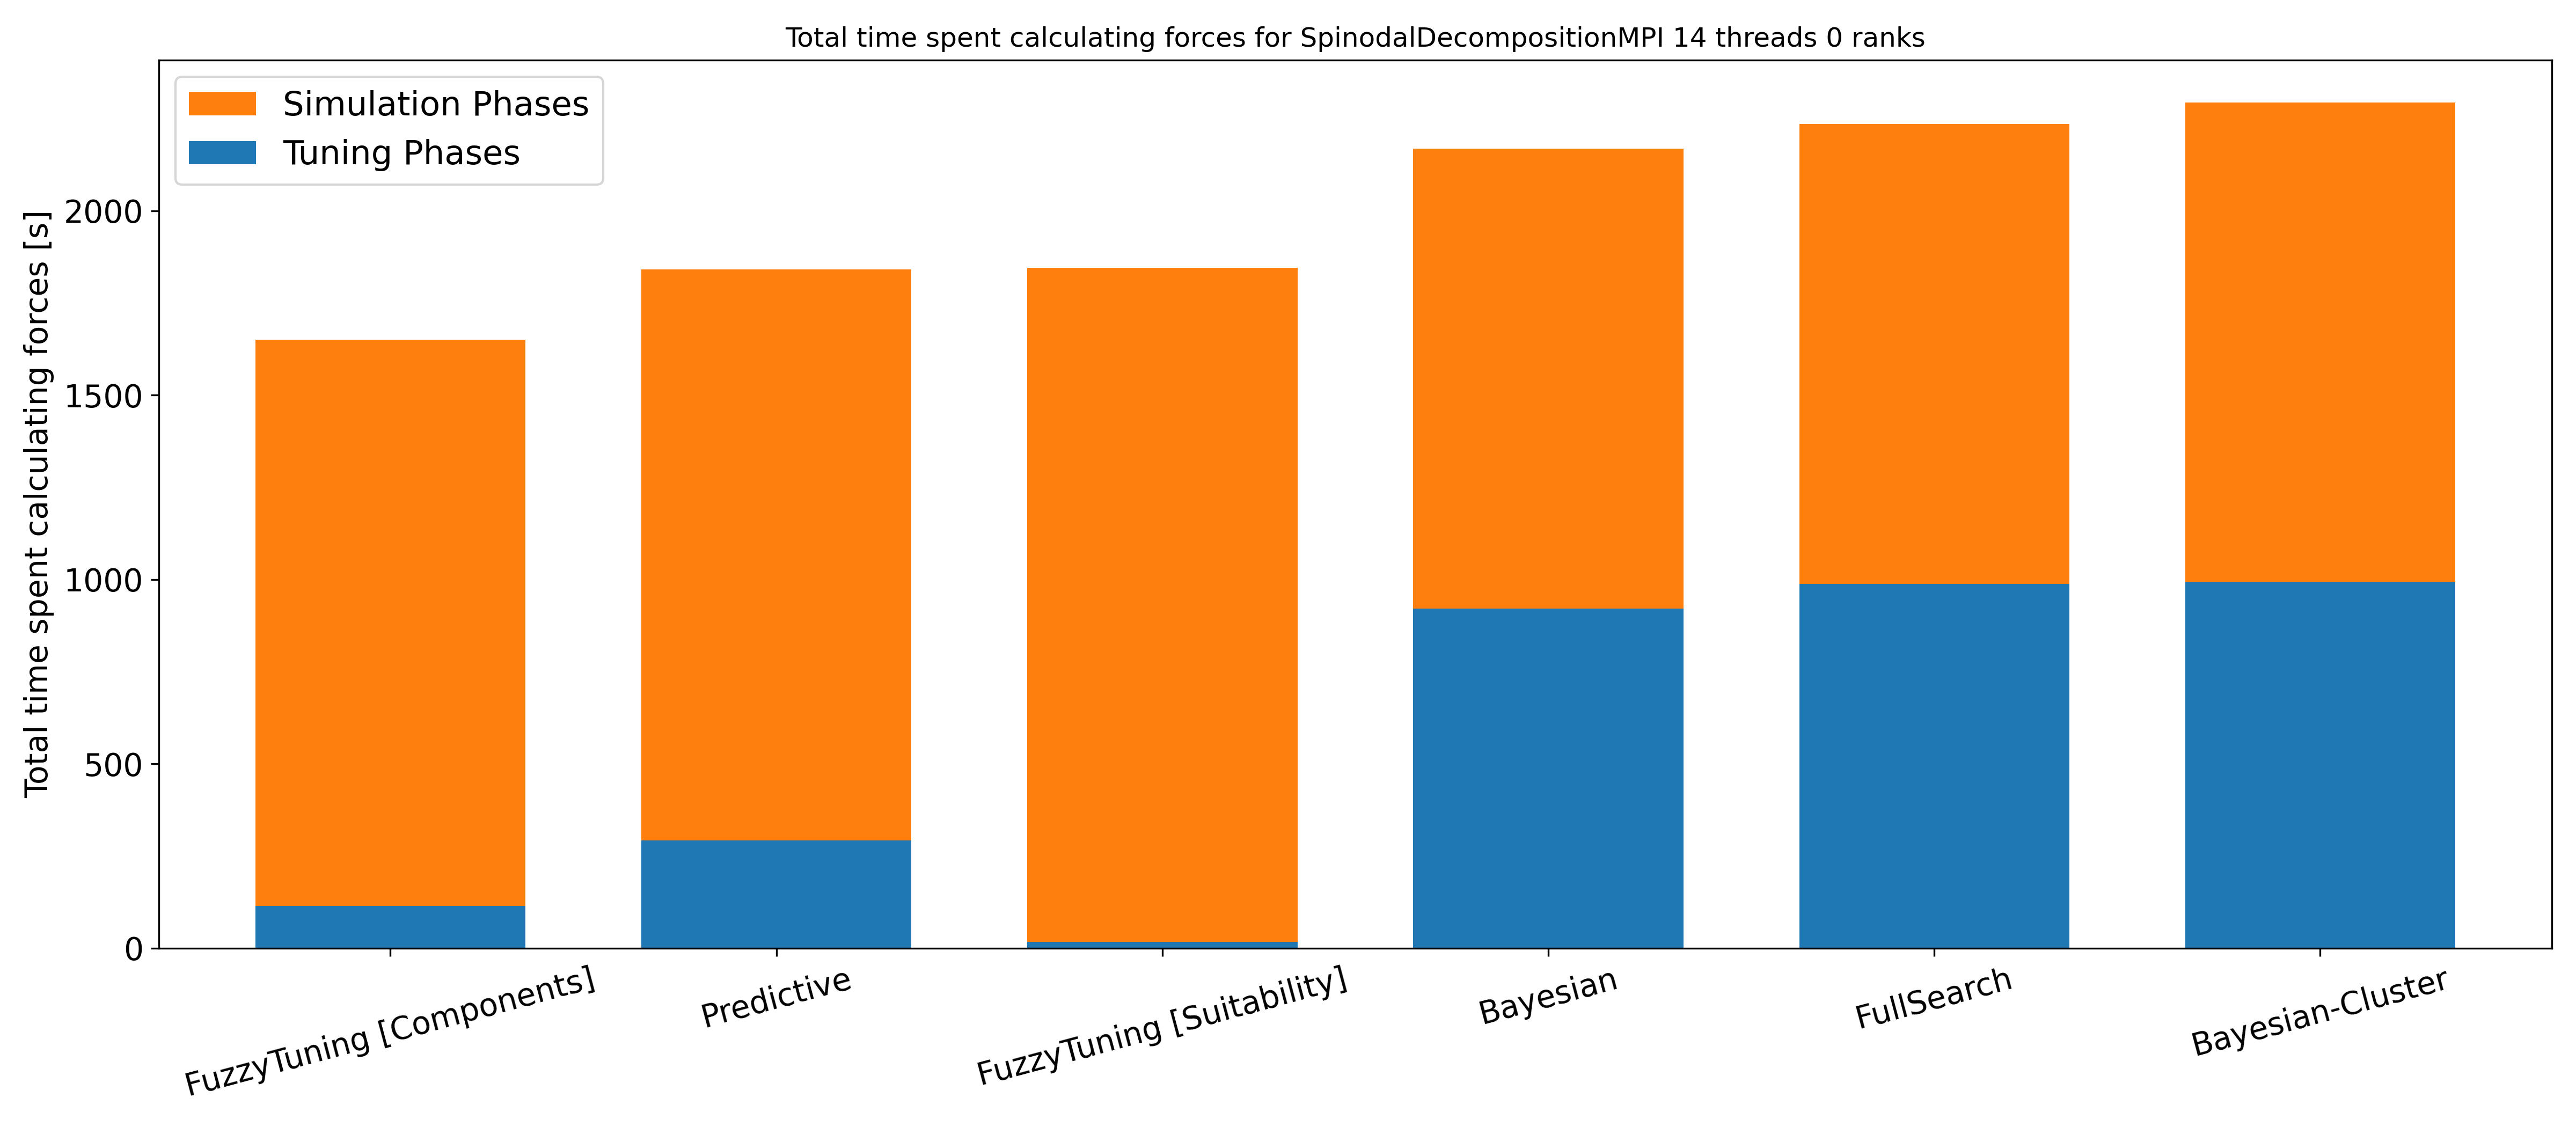
\includegraphics[width=\columnwidth,trim={0cm 0.5cm 0cm 0.9cm},clip]{figures/Benchmark/SpinodalDecompositionMPI/SpinodalDecompositionMPI_timings_total_SpinodalDecompositionMPI_14_0.png}
        \caption{}
        \label{fig:spinodalTotalTime_14thread}
    \end{subfigure}


    \caption[Benchmark Results for the Spinodal Decomposition MPI Scenario]{0th Rank of the Spinodal decomposition benchmark (Total: 4 MPI ranks, 14 threads each). (a) Time spent calculating forces for every iteration. (b) Boxplots of time spent calculating forces divided into tuning- and simulation phases. (c) Total time spent calculating forces for tuning- and simulation phases. The suitability approach uses a non-optimal threshold of 10\% (see \autoref{sec:suitabilityThreshold}).}
    \label{fig:spinodal_14thread}
\end{figure}



\section{Further Analysis}

\subsection{Quality of Predictions During Tuning Phases}

As described above, a tremendous slowdown of the classical tuning strategies is caused by very bad configurations encountered during the tuning phases. To further illustrate this, we will investigate the speedup density distribution of all configurations evaluated during the tuning phases of the different strategies. In particular, we will look at the Exploding Liquid and Spinodal Decomposition MPI scenarios introduced above.

The plots in \autoref{fig:tuningPhaseSpeedup} show the relative speed distributions of all configurations evaluated during the tuning phases.

All classical tuning strategies tend to encounter configurations with extremely low relative speed during the tuning phases. In the exploding-liquid benchmark, some evaluated configurations are up to 10 times slower than the winning configurations, while we observe iterations up to 100 times slower in the Spinodal Decomposition MPI scenario.

The component tuning approach also encounters such bad configurations, but they are less frequent than in the classical tuning strategies and, therefore, do not significantly impact the overall performance.

The suitability approach performs very well in both scenarios, predicting configurations with the highest median relative speed. The high relative speed of the suitability could be caused by the low suitability threshold of 10\%, which caused the strategy to predict only very few configurations, which were all reasonably good. As mentioned previously, we will investigate the impact of the suitability threshold in more detail in \autoref{sec:suitabilityThreshold}.

\subsubsection{Potential Improvement: Early Stopping of Bad Configurations}

As most tuning strategies are plagued by evaluating extremely bad configurations during the tuning phases, it would be highly beneficial to AutoPas if such configurations could be detected during their evaluation and discarded early. Such an improvement could drastically benefit every tuning strategy by significantly reducing the time spent in the tuning phases while still finding the same optimal configuration.

A simple strategy could be aborting a configuration's evaluation if it performs worse than the current best configuration by a certain factor. Additionally, evaluating a configuration can be stopped if it performs worse than the configuration used in the prior simulation phase.

\begin{figure}[H]
    \centering
    \begin{subfigure}[c]{\textwidth}
        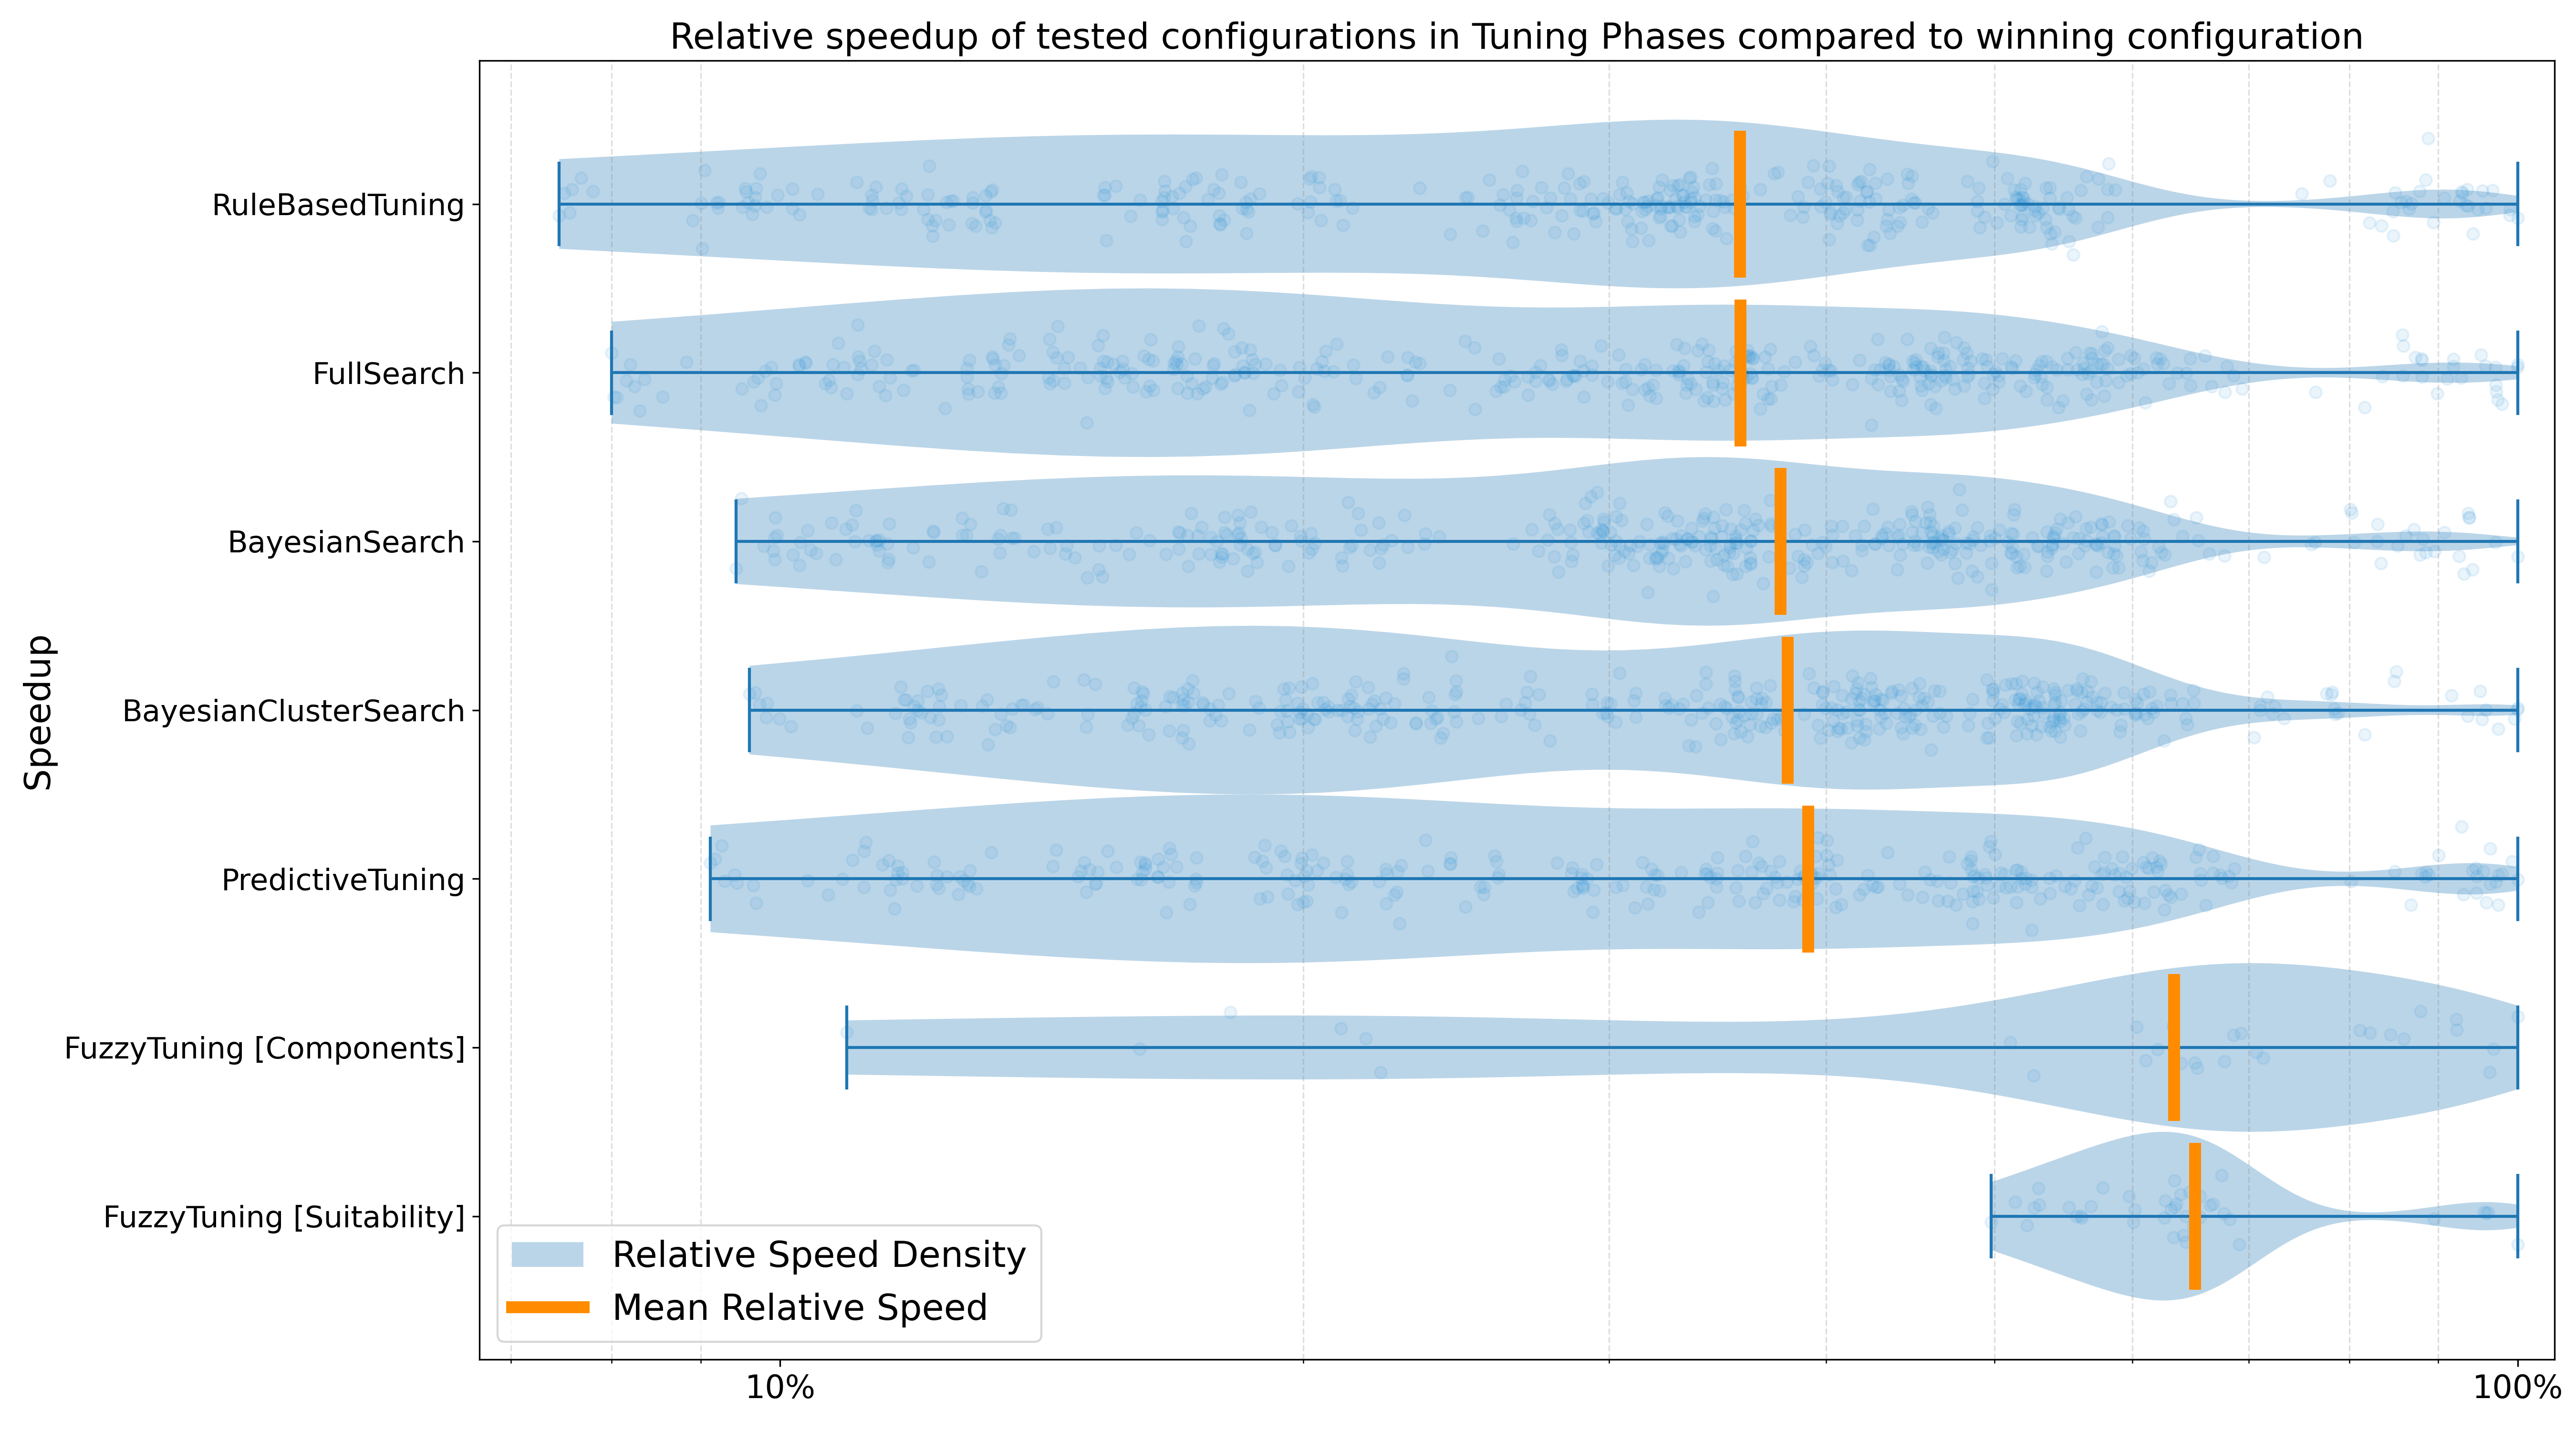
\includegraphics[width=\columnwidth,trim={1cm 0 0cm 1cm},clip]{figures/Benchmark/Observations/tuning_phase_speedup_explodingLiquid_1_zoomed.png}
        \caption{Exploding Liquid scenario with one thread.}
        \label{fig:explodingLiquidSpeedupDensity}
    \end{subfigure}
    \begin{subfigure}[c]{\textwidth}
        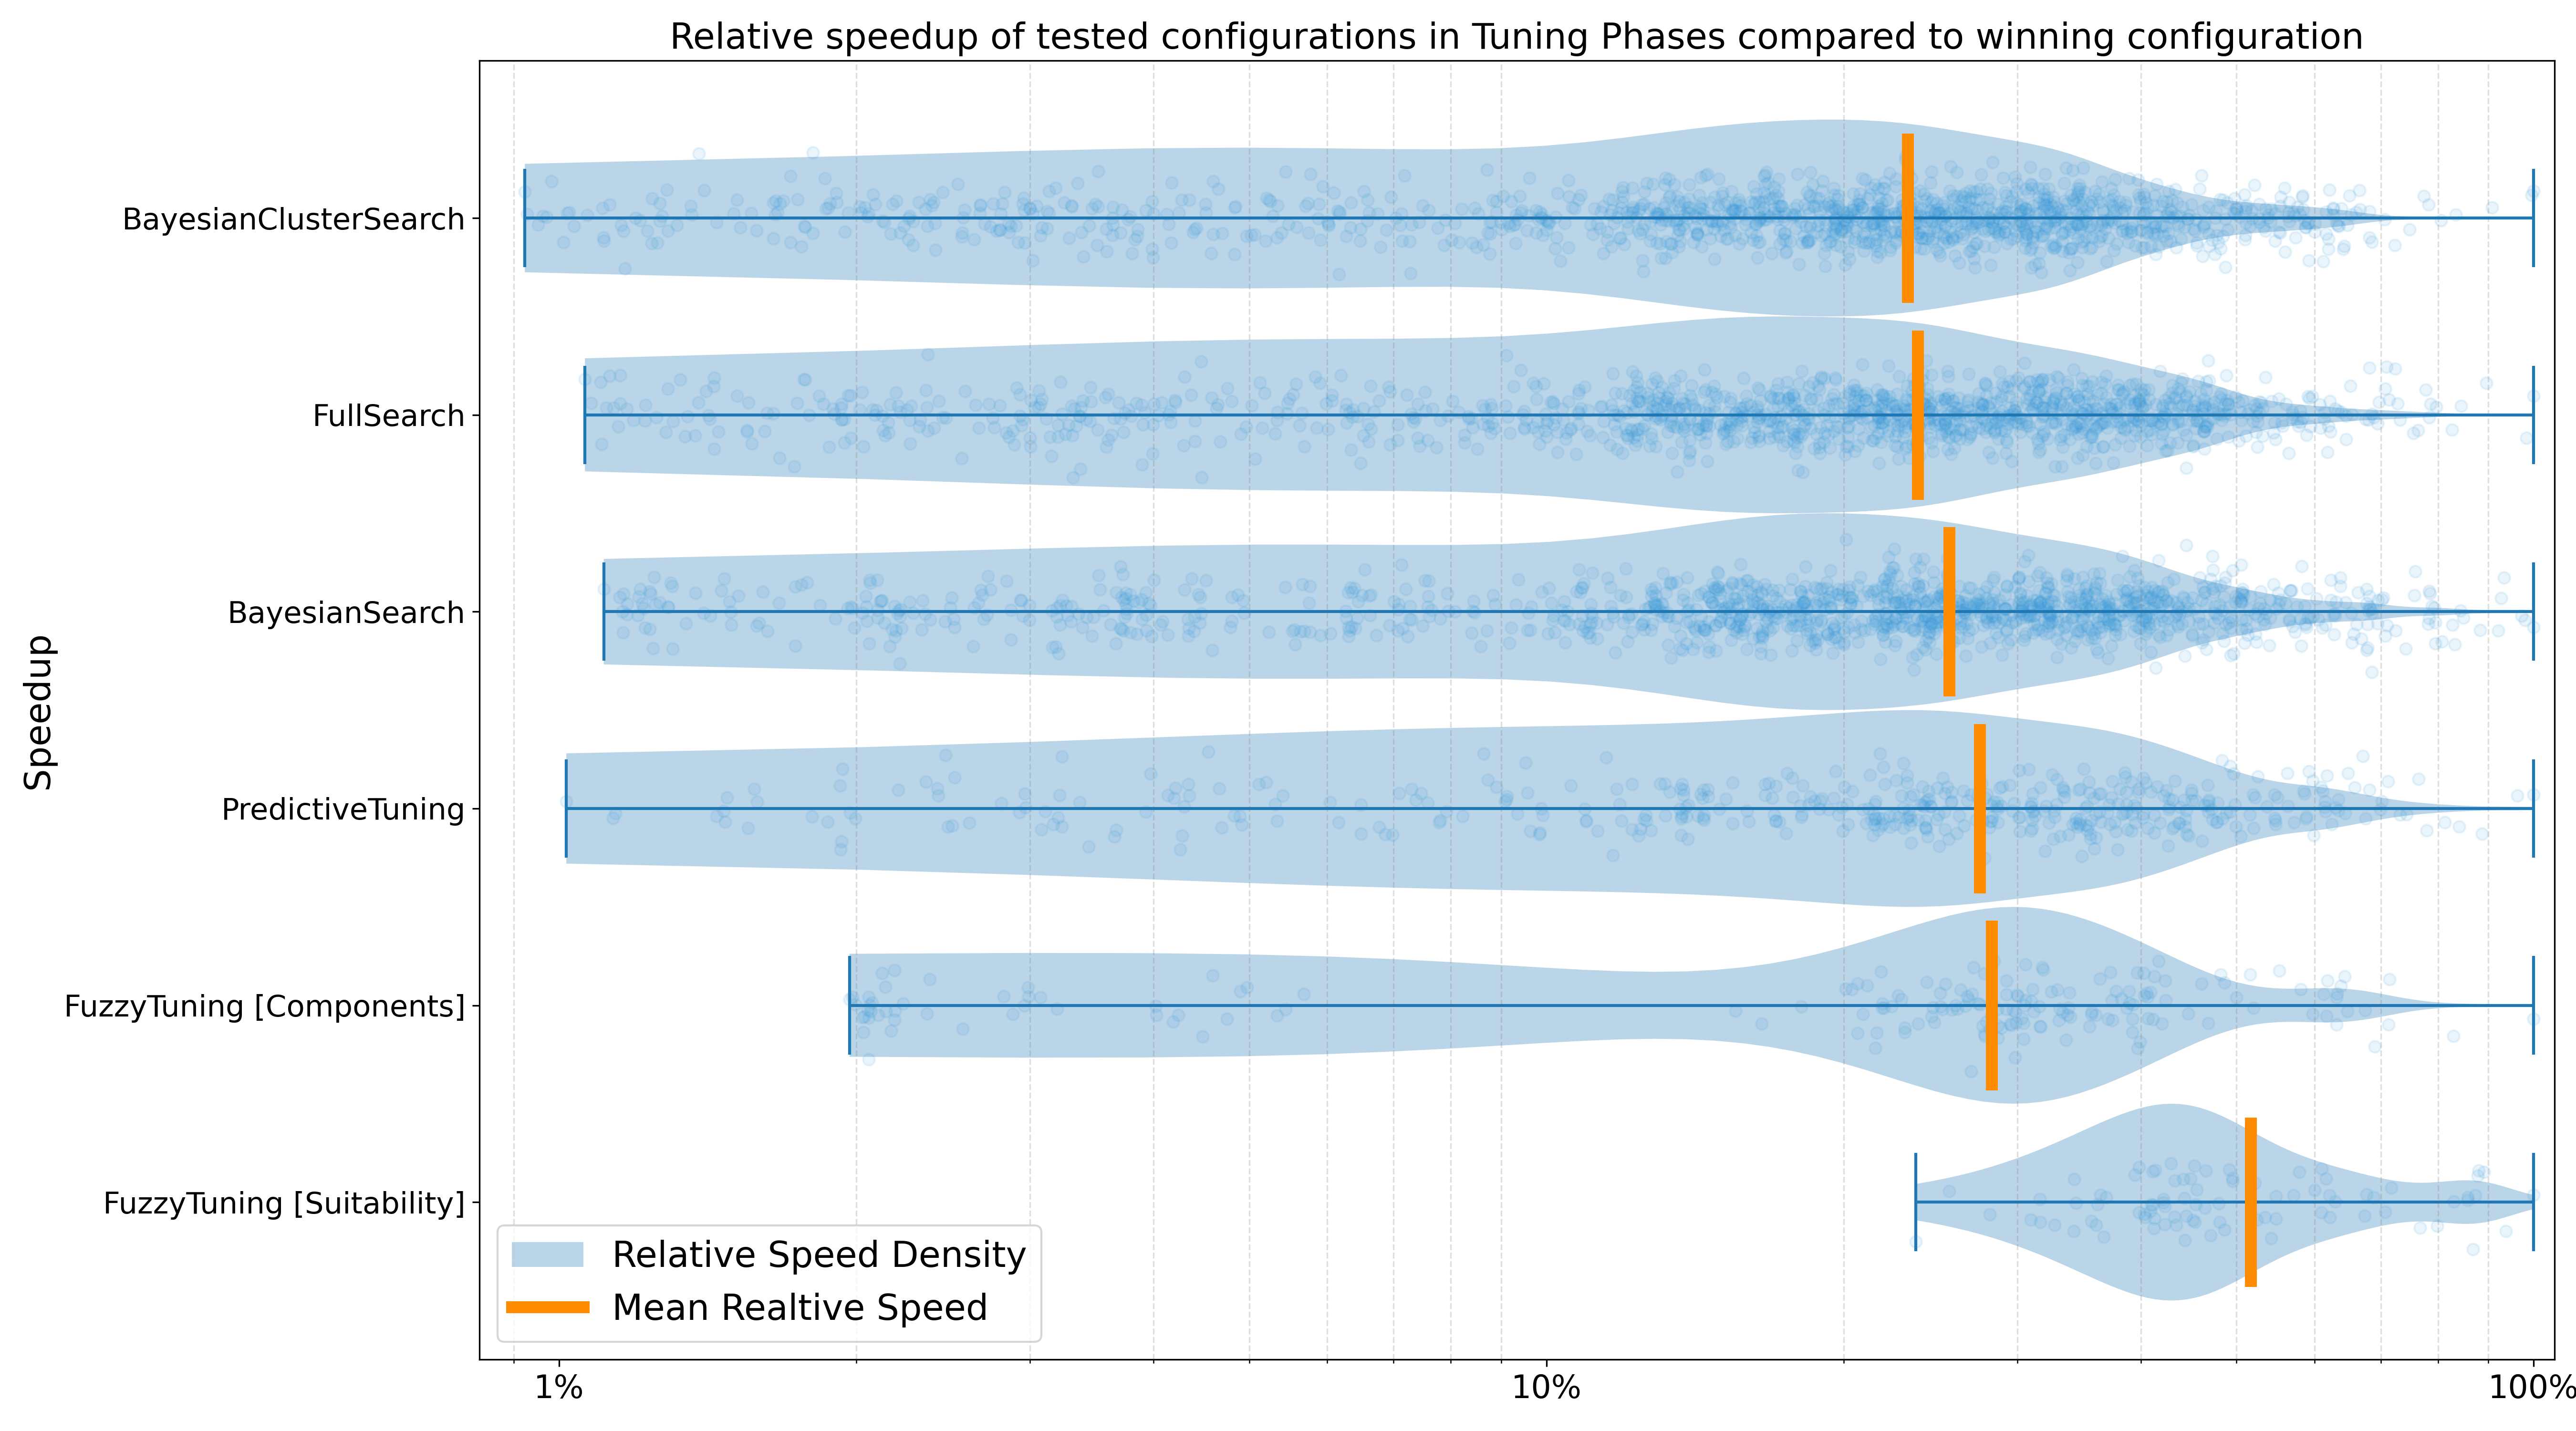
\includegraphics[width=\columnwidth,trim={1cm 0 0cm 1cm},clip]{figures/Benchmark/Observations/tuning_phase_speedup_SpinodalDecompositionMPI_14_0.png}
        \caption{Rank 0 of the Spinodal Decomposition MPI scenario with 14 threads.}
        \label{fig:spinodalSpeedupDensity}
    \end{subfigure}
    \caption[
        Relative speed distribution of configurations evaluated during tuning phases
    ]{The plot shows the relative speed distribution of all configurations evaluated during the tuning phases of both the Exploding Liquid and Spinodal Decomposition MPI scenarios calculated from the smoothed timings (see \autoref*{des:tuningdatafields}). The fuzzy tuning strategies generally encounter better configurations during the tuning phases, which improves their total performance.}
    \label{fig:tuningPhaseSpeedup}
\end{figure}

\subsection{Optimal Suitability Threshold}
\label{sec:suitabilityThreshold}

In previous measurements, the Component tuning approach performed better than the Suitability tuning approach, mainly due to the suitability approach not finding the optimal configuration during the tuning phases (see \autoref{fig:spinodalTimings_14thread}).

The previous benchmarks were executed with a rule file specifying that only the top 10\% of configurations with the highest suitability should be selected, which may have been too low, causing a high chance of not finding the globally optimal configuration.

To investigate this issue, we reran the Exploding Liquid benchmark with different suitability thresholds each time, measuring the total runtimes as shown in \autoref{fig:suitabilityThreshold}.

From the figure, we observe that very low thresholds perform poorly, as they select too few configurations for the tuning phases, resulting in a high chance of not including the optimal configuration. Very high thresholds also perform poorly, as high suitability values cause the strategy to behave like FullSeach, selecting nearly all configurations to be evaluated.

The optimal suitability threshold for this scenario lies between 20\% and 40\%, which guarantees that the best configuration is selected for the tuning phases while still keeping the total number of evaluated configurations low. Following this observation, we updated the default value of the rule file of the suitability approach to 30\%. This change should improve the suitability approach's performance in future benchmarks.

\begin{figure}[H]
    \centering
    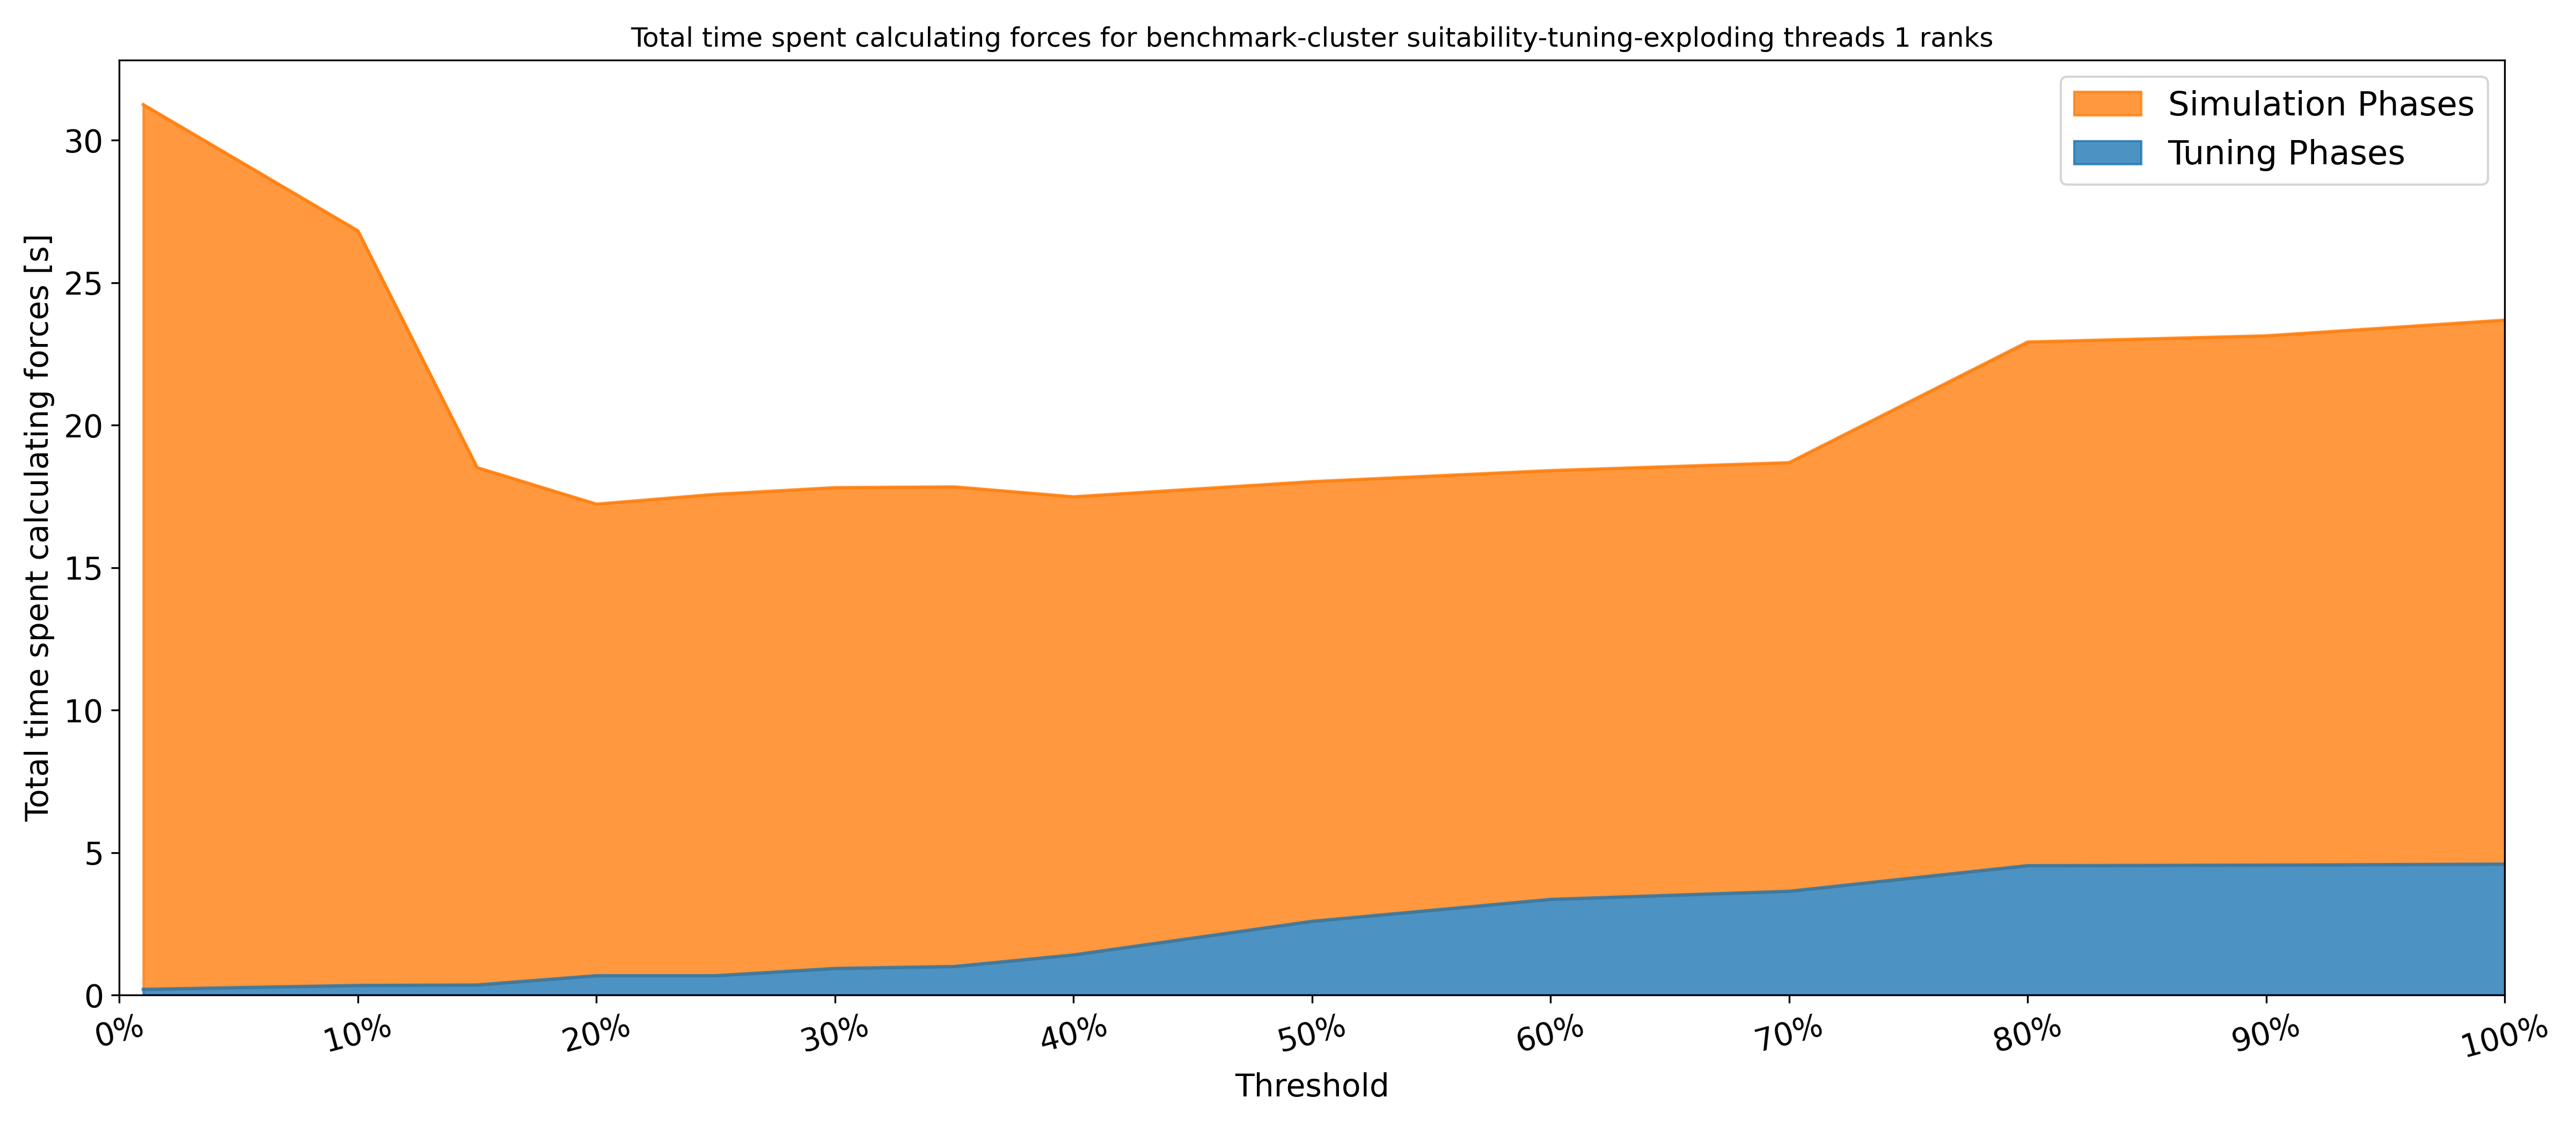
\includegraphics[width=\columnwidth,trim={0cm 0cm 0cm 0.9cm},clip]{figures/Benchmark/SuitabilitySearch/SuitabilityExploding_timings_threshold_benchmark-cluster_suitability-tuning-exploding_1.png}
    \caption[
        Impact of the suitability threshold on the simulation performance
    ]{Exploding liquid benchmark with different suitability thresholds. The fastest runtimes are achieved with a threshold between 20\% and 40\%. The time spent calculating forces during tuning phases increases with higher thresholds as the strategy converges towards the behavior of FullSearch.}
    \label{fig:suitabilityThreshold}
\end{figure}

\newpage

\subsection{Generalization of Rule Extraction}

Previous measurements of the Exploding Liquid and the Spinodal Decomposition MPI benchmark showed that the fuzzy tuning strategies perform well. However, all previously tested scenarios were in some way included in the training data, which could have biased the results in favor of the fuzzy tuning strategies.

To investigate the generalization of the rule extraction process, we reran the rule extraction process without the Exploding Liquid scenario in the training data.

We reran the Exploding Liquid benchmark with the new rule files, named \emph{holdout} rule files, to see if the fuzzy tuning strategies can still perform well even without the scenario being included in the training data.

The results in \autoref{fig:explodingTimings_1thread_noTrainingData} show that the fuzzy tuning strategies still perform remarkably well, with comparable performance to the previous measurements. The remaining training scenarios provided enough general tuning information to still allow the fuzzy tuning strategies to perform the best in the Exploding Liquid scenario.

Therefore, we conclude that the rule extraction process is reasonably robust, and the extracted rules can be generalized to similar scenarios, even if they were not included in the training data.

\begin{figure}[H]
    \centering
    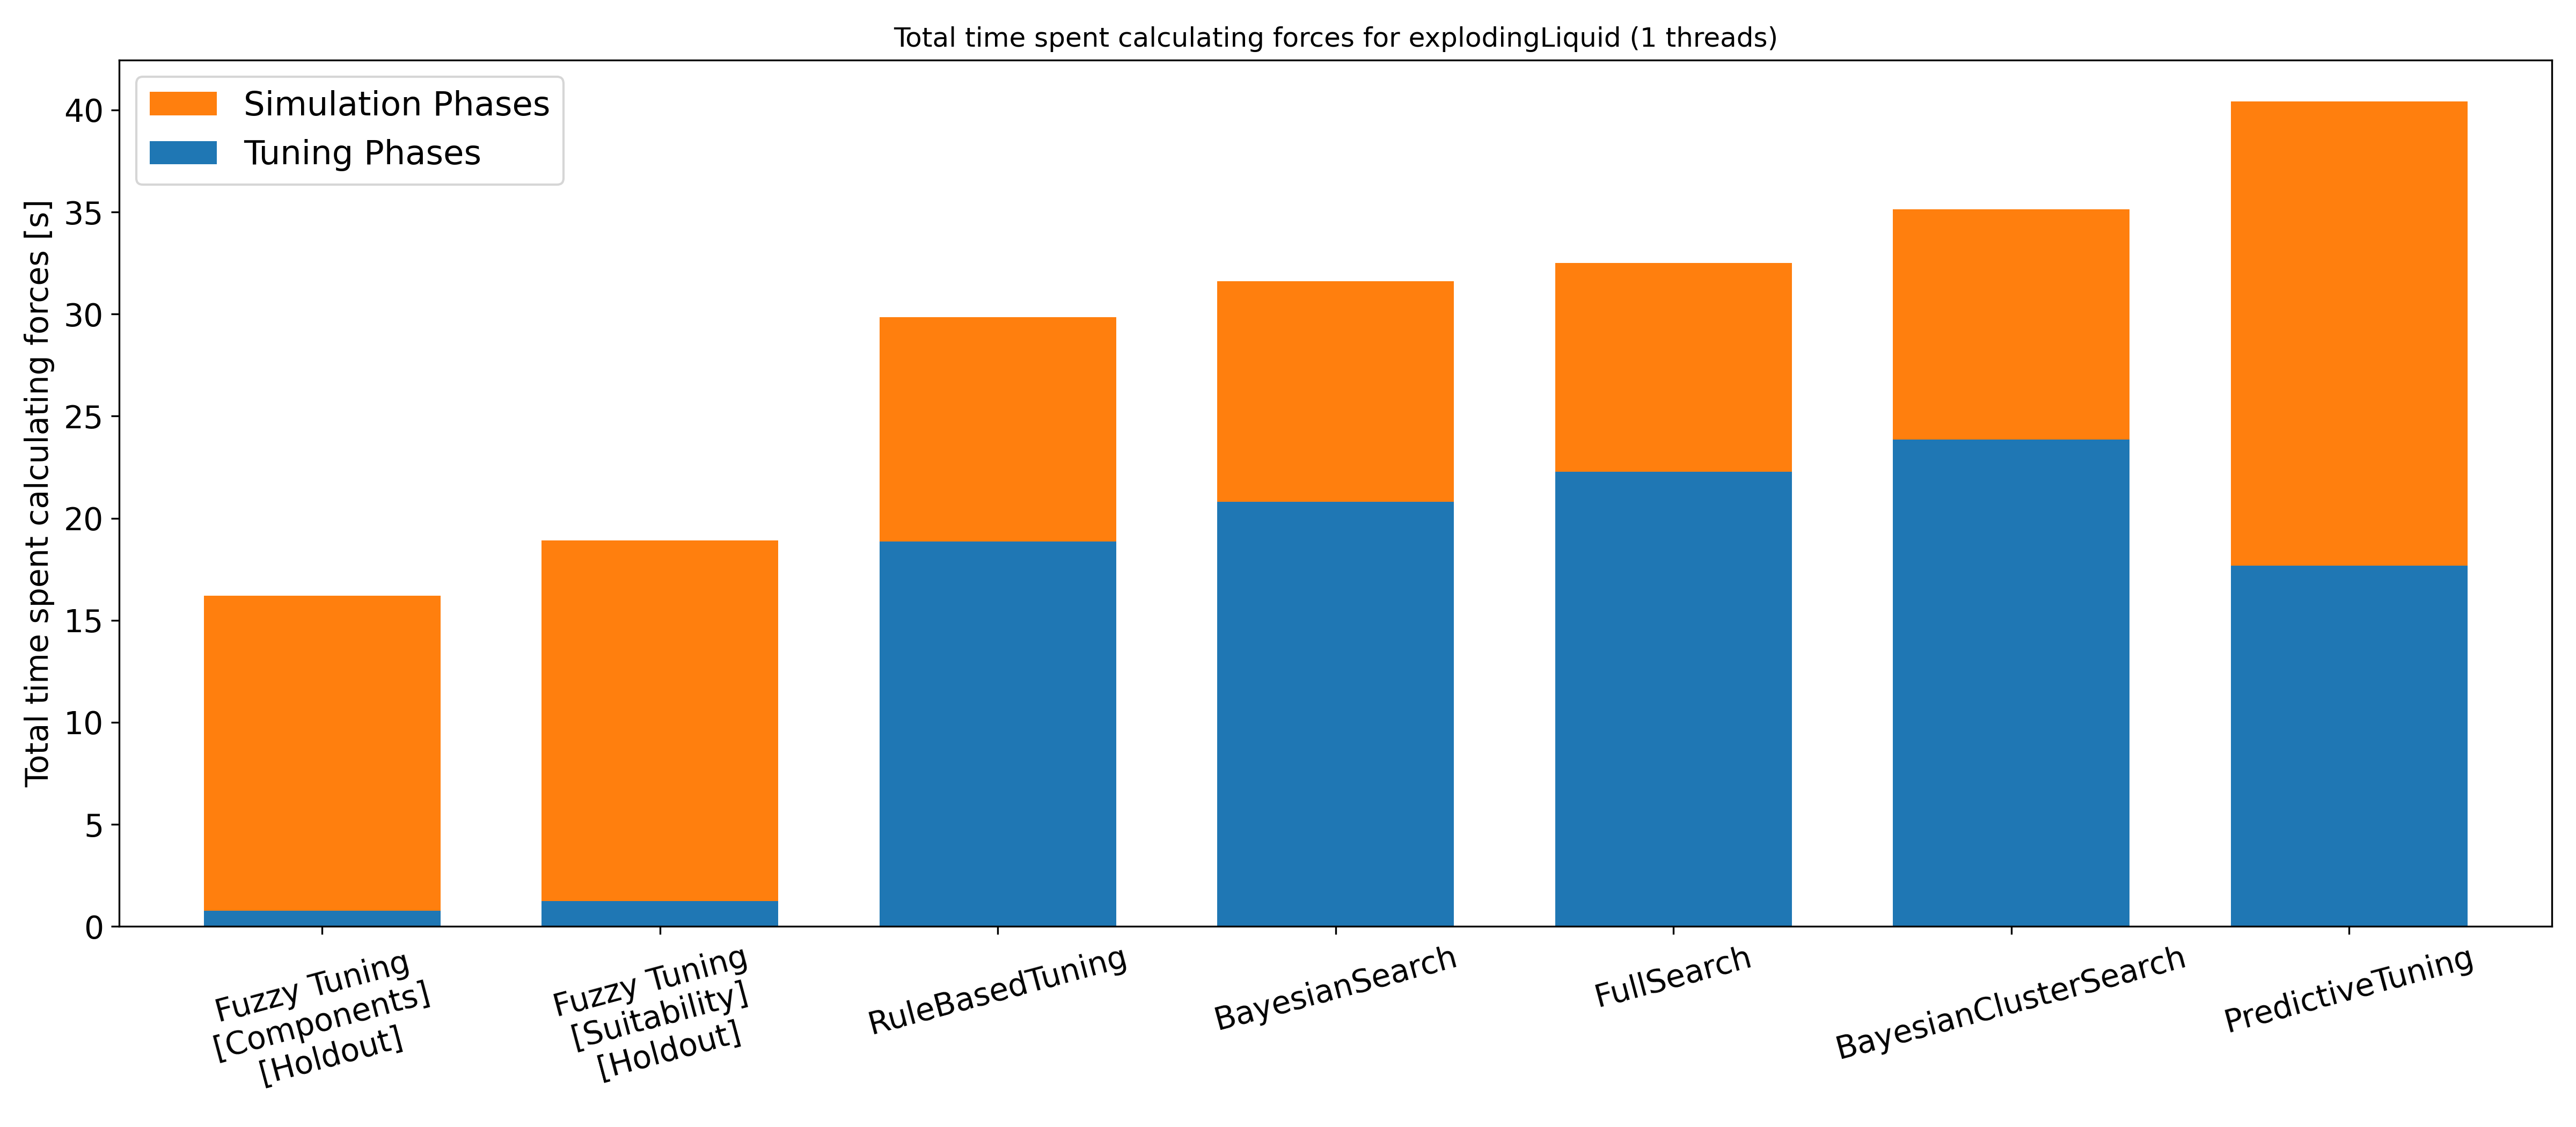
\includegraphics[width=\columnwidth,trim={0cm 0 0cm 0.9cm},clip]{figures/Benchmark/ExplodingLiquidHoldout/total_time_explodingLiquid_1.png}
    \caption[
        Benchmark Results for the Exploding Liquid Scenario (Holdout)
    ]{
        Total time spent calculating forces for tuning- and simulation phases for the Exploding Liquid benchmark without the scenario being included in the training data. The fuzzy tuning strategies still perform best and are comparable to the previous measurements.
    }
    \label{fig:explodingTimings_1thread_noTrainingData}
\end{figure}